\documentclass{article}
\usepackage{graphicx} 
\usepackage{float}
\usepackage{booktabs}
\usepackage{array}
\usepackage{arydshln}
\usepackage{siunitx}
\usepackage{cancel}
\usepackage{changepage}
\usepackage{placeins}
\usepackage{enumitem}
\usepackage{siunitx}
\usepackage{lipsum}
\usepackage[most]{tcolorbox}
\definecolor{light-gray}{gray}{0.9}
\newcommand{\code}[1]{\colorbox{light-gray}{\texttt{#1}}}
\usepackage{subcaption}


%\usepackage{showframe}
\usepackage{times}

\DeclareSIUnit{\atm}{atm}

\usepackage{tabularx}
\usepackage{amsmath, amssymb, amscd, MnSymbol, mathrsfs}
\usepackage{cellspace}
\usepackage{tikz}
\usetikzlibrary{calc,3d, patterns, angles, quotes, decorations.markings, decorations.pathmorphing, hobby}
\usepackage{xfrac}

\usepackage{chemfig}
\usepackage{caption}
\usepackage{bm}

\usepackage{pdfpages}
\usepackage{pdflscape}
\usepackage{afterpage}

\usepackage{empheq}
\usepackage{pgfplots}
\usepackage{pgfplotstable}
\usepackage{xstring}

\pgfplotsset{compat=1.18}


\usepackage[european,americanvoltages,americanresistors,cuteinductors,fetbodydiode]{circuitikz}
\usetikzlibrary{circuits.logic.US}
\usepackage{siunitx}
\usetikzlibrary{arrows,shapes,calc, positioning, patterns, decorations, decorations.markings}
\usetikzlibrary{positioning}
\usetikzlibrary{calc}
%\ctikzset{bipoles/thickness=1}
%\tikzstyle{every node}=[font=\small]
%\tikzstyle{every path}=[line width=0.8pt,line cap=round,line join=round]

\def\CalcC#1{%
	\coordinate (base) at (#1.base);
	\coordinate (collector) at (#1.collector);
	\coordinate (emitter) at (#1.emitter);
	\draw (barycentric cs:base=0.5,collector=0.5,emitter=0.5) circle [radius=14pt];
}

\usepackage{tikz-3dplot}
\usepackage{textcomp}
% Custom commands
\newcommand{\vect}[1]{\boldsymbol{\mathbf{#1}}}
\newcolumntype{C}{>{\centering\arraybackslash}X}
\newcolumntype{M}[1]{>{\centering\arraybackslash}m{#1}}

%\usetikzlibrary{external}
%\tikzexternalize[prefix=figures/]

\newcommand\myfrac[2]{\sfrac{#1\mkern-1.2mu}{#2}}
\usepackage{xcolor}

% Define custom colors
\definecolor{darkblue}{rgb}{0.1,0.1,0.5} %  dark blue shade
\definecolor{formalshade}{rgb}{0.95,0.95,1} % light blue shade for the background

% For the adjustwidth environment
\PassOptionsToPackage{strict}{changepage}
\usepackage{changepage}

% For formal definitions
\usepackage{framed}

\newcommand{\formalsource}{} % Initialize an empty macro to store the source text

\newenvironment{formal}[3][]{% Start of the environment
	\renewcommand{\formalsource}{#1}% Store the optional argument
	\def\FrameCommand{%
		\hspace{1pt}%
		{\color{#2}\vrule width 2pt}%
		{\color{#3}\vrule width 4pt}%
		\colorbox{#3}%
	}%
	\MakeFramed{\advance\hsize-\width\FrameRestore}%
	\noindent\hspace{-4.55pt}% Disable indenting the first paragraph
	\begin{adjustwidth}{}{7pt}%
		\vspace{2pt}%
	}%
	{%
		\vspace{4pt}%
		\ifx\formalsource\empty % Check if the source is empty
		\else
		\hfill{\footnotesize{\formalsource}}% Align source to the bottom-right
		\fi
	\end{adjustwidth}\endMakeFramed%
}


% Custom itemize list with images for positive and negative items
\newlist{gitemize}{itemize}{1} % Just one level for the list
\setlist[gitemize,1]{
	leftmargin=2.8em, % Adjust the margin for the list
	labelsep=1em % Control the space between the label and the list item
}

% Define checkmark and cross symbols for positive and negative items
\newcommand{\checkitem}{\raisebox{-0.25\height}{\includegraphics[width=0.4cm]{checkmark.png}}}
\newcommand{\crossitem}{\raisebox{-0.25\height}{\includegraphics[width=0.4cm]{cross.png}}}


\usepackage[left=0.8in,right=0.8in,top=0.5in,bottom=0.69in,includeheadfoot,letterpaper]{geometry}
\usepackage{fancyhdr}
\usepackage{hyperref}
\usepackage{graphicx}
\usepackage{tabularray}
\usepackage{varwidth} 


\newcommand{\wm}[2]{%
	\begin{minipage}{#1\textwidth}
		\centering
		#2
	\end{minipage}%
}

\pagestyle{fancy}
\fancyhf{}


\renewcommand{\headrulewidth}{0.4pt}
\renewcommand{\footrulewidth}{0.4pt}

\fancyhead[L]{
\includegraphics[height=1.2cm]{images/Kingston_University_London_logo_200-tablet.png}}
\fancyhead[R]{EG4023 – ME – IMechE Design Challenge Project}
\fancyfoot[C]{Department of Mechanical Engineering}
\fancyfoot[R]{\thepage}

\usepackage{scalerel}
\usepackage{pythonhighlight}
\setlength{\headheight}{30pt}
\setlength{\footskip}{20pt}



\usepackage[export]{adjustbox}
\usepackage{tocloft}
\renewcommand{\cfttoctitlefont}{}
\renewcommand{\contentsname}{}
\renewcommand{\cftsecleader}{\cftdotfill{\cftdotsep}}

\setlength{\cftbeforesecskip}{0.5em}



\usepackage{hyperref}    % For hyperlinks
\usepackage{xurl}        % For better URL handling
\hypersetup{
	colorlinks=true,
	linkcolor=blue!50!black,
	urlcolor=blue,       % Color for URLs
}


\definecolor{ChineseGold}{HTML}{C59401}
\definecolor{AmericanGold}{HTML}{D3AF37}
\definecolor{MetallicSunburst}{HTML}{A77C37}
\definecolor{GoldenBrown}{HTML}{996515}
\definecolor{DarkBrown}{HTML}{674222}
\definecolor{SkyBlue}{HTML}{87CEEB}      % Soft and bright
\definecolor{BabyBlue}{HTML}{89CFF0}     % Gentle, pastel-like
\definecolor{SteelBlue}{HTML}{4682B4}    % Rich but not overpowering
\definecolor{RoyalBlue}{HTML}{4169E1}    % Strong, slightly purplish
\definecolor{MidnightBlue}{HTML}{191970} % Almost black, deep navy
\definecolor{PrussianBlue}{HTML}{003153} % Very deep blue with a classic look
\definecolor{mainblue}{HTML}{1D73BE}

\usepackage{listings}

\definecolor{codegreen}{rgb}{0,0.6,0}
\definecolor{codegray}{rgb}{0.5,0.5,0.5}
\definecolor{codepurple}{rgb}{0.58,0,0.82}
\definecolor{backcolour}{rgb}{0.95,0.95,0.92}

\lstdefinestyle{mystyle}{
	backgroundcolor=\color{white!97!gray},   
	commentstyle=\color{codegreen},
	keywordstyle=\color{purple},
	numberstyle=\tiny\color{codegray},
	stringstyle=\color{orange},
	basicstyle=\ttfamily\scriptsize,
	breakatwhitespace=false,         
	breaklines=true,                 
	captionpos=b,                    
	keepspaces=true,                 
	numbers=left,                    
	numbersep=5pt,                  
	showspaces=false,                
	showstringspaces=false,
	showtabs=false,                  
	tabsize=2
}

\lstset{style=mystyle}

%Refer to the equation as \eqref{equation}.
\usepackage{caption}  % This package allows captioning outside of a float
\usepackage[export]{adjustbox}


\usetikzlibrary{patterns}

\usetikzlibrary{patterns.meta}
\usepackage[para]{footmisc} % Example of making footnotes run together in a paragraph

\definecolor{darkgreen}{rgb}{0.0, 0.5, 0.0}

\usepackage{datetime}

\usepackage{etoolbox}
\AfterEndEnvironment{landscape}{\clearpage\restoregeometry}

\makeatletter
\def\tagform@#1{\maketag@@@{{Eq.~#1}}} 
\makeatother

\usepackage{ifthen}
\usepackage{calc}
\usepackage{datenumber}

\usepackage{physics}
\usepackage[outline]{contour}
\usetikzlibrary{patterns,decorations.pathmorphing}
\usetikzlibrary{arrows.meta}
\tikzset{>=latex}
\contourlength{1.1pt}

\colorlet{mydarkblue}{blue!50!black}
\colorlet{myred}{red!65!black}
\colorlet{watercol}{blue!80!cyan!10!white}
\colorlet{darkwatercol}{blue!80!cyan!20!white}
\tikzstyle{piston}=[blue!50!black,top color=blue!30,bottom color=blue!50,middle color=blue!20,shading angle=0]
\tikzstyle{water}=[draw=mydarkblue,top color=watercol!90,bottom color=watercol!90!black,shading angle=5]
\tikzstyle{vertical water}=[water,
top color=watercol!90!black!90,bottom color=watercol!90!black!90,middle color=watercol!80,shading angle=90]
\def\tick#1#2{\draw[thick] (#1)++(#2:0.1) --++ (#2-180:0.2)}



\newcounter{deadlineyear}\setcounter{deadlineyear}{2025}
\newcounter{deadlinemonth}\setcounter{deadlinemonth}{4}
\newcounter{deadlineday}\setcounter{deadlineday}{9}
\newcounter{deadlinetime}\setcounter{deadlinetime}{1439} % Default: 23:59 (1439 minutes)
\newcounter{mydatenumber}
\newcounter{currentdate}
\newcounter{daysdiff}
\newcounter{currenttime}
\newcounter{totalminutes}
\newcounter{displaydays}
\newcounter{remainingmins}
\newcounter{displayhours}
\newcounter{displaymins}

% ====== MACROS ======
% Set deadline time (e.g., \setdeadlinetime{23}{59})
\newcommand{\setdeadlinetime}[2]{%
	\setcounter{deadlinetime}{#1 * 60 + #2}%
}

% Main calculation command
\newcommand{\timeUntilDeadline}{%
	% Calculate days between dates
	\setmydatenumber{mydatenumber}{\thedeadlineyear}{\thedeadlinemonth}{\thedeadlineday}%
	\setmydatenumber{currentdate}{\the\year}{\the\month}{\the\day}%
	\setcounter{daysdiff}{\themydatenumber - \thecurrentdate}%
	
	% Get current time in minutes since midnight
	\setcounter{currenttime}{\time}%
	
	% Calculate total remaining minutes (deadline time - current time)
	\setcounter{totalminutes}{\thedaysdiff * 1440 + \thedeadlinetime - \thecurrenttime}%
	
	% Check deadline status
	\ifnum\thetotalminutes < 0
	\textbf{\color{red}Deadline passed!}%
	\else
	% Calculate time components
	\setcounter{displaydays}{\thetotalminutes / 1440}%
	\setcounter{remainingmins}{\thetotalminutes - \thedisplaydays * 1440}%
	\setcounter{displayhours}{\theremainingmins / 60}%
	\setcounter{displaymins}{\theremainingmins - \thedisplayhours * 60}%
	
	% Format output
	\textbf{%
		\ifnum\thedisplaydays > 0
		\thedisplaydays\ day\ifnum\thedisplaydays > 1 s\fi%
		\ifnum\thedisplayhours > 0
		\ifnum\thedisplaymins > 0, \else\ and \fi%
		\else
		\ifnum\thedisplaymins > 0\ and \fi%
		\fi%
		\fi%
		\ifnum\thedisplayhours > 0
		\thedisplayhours\ hour\ifnum\thedisplayhours > 1 s\fi%
		\ifnum\thedisplaymins > 0\ and \fi%
		\fi%
		\ifnum\thedisplaymins > 0
		\thedisplaymins\ minute\ifnum\thedisplaymins > 1 s\fi%
		\fi%
		\ left%
	}%
	\fi
}

\definecolor{mygreen}{HTML}{07a56d}

\newtcbtheorem{briefillus}{Definiton}{
	enhanced,
	sharp corners,
	attach boxed title to top left={
		xshift=0pt, 
		yshift=-\tcboxedtitleheight, 
		yshifttext=-\tcboxedtitleheight/2-0.5em
	},
	colback=white,
	colframe=black,
	fonttitle=\bfseries,
	coltitle=white,
	boxed title style={
		rounded corners,
		arc=2pt,
		size=small,
		colback=black,
		colframe=black,
	},
	leftrule=0pt, 
	rightrule=0pt, 
}{thm}

\usepackage{titlesec}

\titleformat{\section}[block]{\vspace*{-15pt}\normalfont\LARGE\bfseries\color{mainblue}}{\color{mainblue}\thesection}{1em}{}
\titleformat{\subsection}[block]{\normalfont\large\bfseries\color{mainblue}}{\color{mainblue}\thesubsection }{1em}{}
\titleformat{\subsubsection}[block]{\normalfont\normalsize\bfseries\color{mainblue}}{\color{mainblue}\thesubsubsection}{1em}{}

\begin{document}

\thispagestyle{empty}

\color{white}
\tikz[remember picture,overlay] \node[opacity=1,inner sep=0pt] at (current page.center){
\includegraphics[width=\paperwidth,height=\paperheight]{images/A4-document-placeholder-medium-blue_0.jpg-ezgif.com-webp-to-jpg-converter(2).jpg}};

\vspace*{\fill}
\begin{center}
	\textbf{\Huge IMechE Design Challenge}\\[10pt]
	\LARGE \textbf{Group Report and Logbook}
\end{center}
\vspace*{\fill}

\Large    
\begin{tabular}{@{}l l l@{}}
	\textbf{Submitted by:}  & Samatar Ahmed (Group Leader) \phantom{ssssssssss}& K2374854\\
	& Sakariye Abiikar & K2371673 \\
	& Jayden Balgobind & K2421484\\
	& Hector Huser & K2367380\\
	& Hashaam Khan & K2371729\\
	& Josh Mossman & K2457119\\
\end{tabular}

\vspace*{\fill}

\begin{tabular}{@{}l l@{}}
	\textbf{Key Dates:} & Date of practical: Thursday 3$^{\text{rd}}$ April, 2025 \\
	& Deadline: Wednesday 9$^{\text{th}}$ April, 2025 23:59\\
	& Last Updated: \today\, \currenttime \\
	& Days left until deadline: \timeUntilDeadline \\
\end{tabular}
\vspace*{\fill}

\large
\newpage\thispagestyle{empty}\newgeometry{top=0.7in,bottom=0.6in,left=0.8in,right=0.8in}
\tikz[remember picture,overlay] \node[opacity=0.5,inner sep=0pt] at (current page.center){
\includegraphics[width=\paperwidth,height=\paperheight]{images/a13d25fa5178ce400e90e65f61d696d3.jpg}};

\color{black}
\vspace*{\fill}
\noindent
\begin{tblr}{
		colspec={Q[5.4cm]Q[5.4cm]Q[5.4cm]},
		hlines,vlines,
		cells={valign=m,halign=c},
		rows={ht=2\baselineskip},
		row{1}={ht=1\baselineskip,font=\bfseries,fg=mainblue!90!white},
	}
	MODULE NO. & MODULE TITLE & MODULE LEADER \\
	EG4023 & Introduction to Engineering Design and Manufacture & Dr Andy Curley \\\hline
	Assignment Title: & \SetCell[c=2]{c} IMechE Design Challenge Project --- Group Report and Logbook &  \\	
\end{tblr}\\[1em]
\begin{tblr}{
		colspec={Q[5.4cm]Q[11.24cm]},
		hlines,vlines,
		cells={valign=m,halign=c},
		rows={ht=2\baselineskip},
	}
	Group Name: & Group 1  \\
\end{tblr}\\[1em]
\begin{minipage}{0.98\textwidth}
	\vspace*{0.1mm}
	\begin{center}
		\fbox{
			\begin{minipage}[c][16cm][c]{\textwidth}\hspace*{1.3em}\vspace*{2em}
				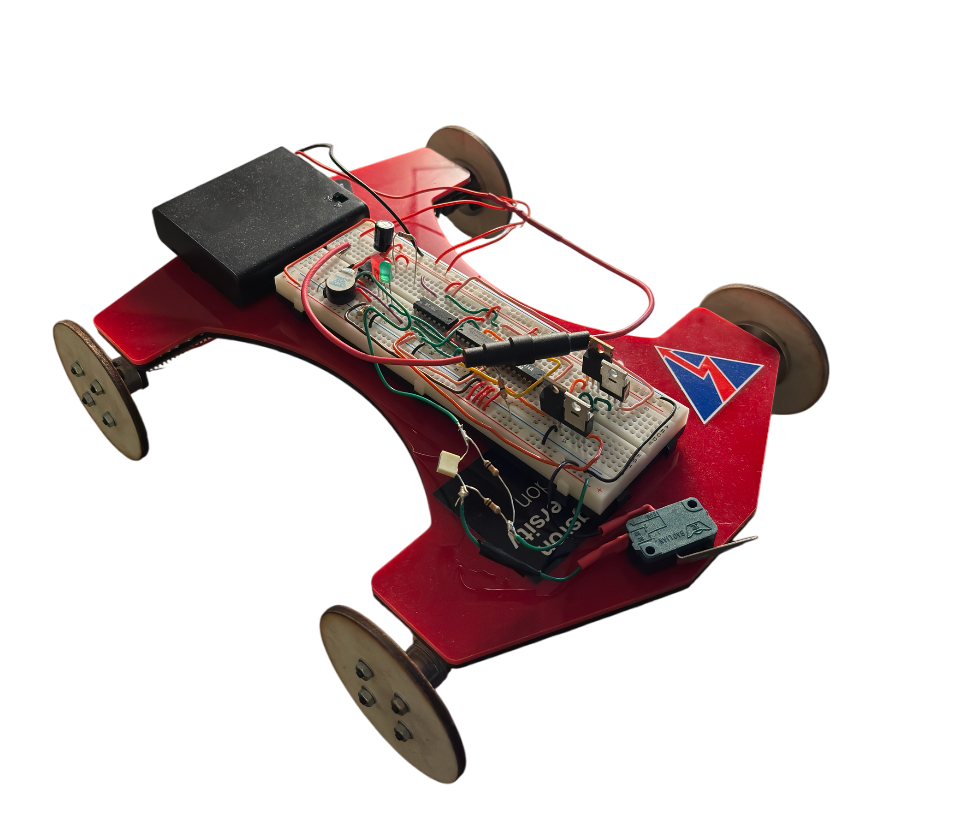
\includegraphics[height=14cm,width=1\textwidth]{images/Image-Photoroom(1).png}
			\end{minipage}
		}
	\end{center}
	\vspace*{1em}
\end{minipage}
\vspace*{\fill}


\newpage\thispagestyle{empty}

\tikz[remember picture,overlay] \node[opacity=0.5,inner sep=0pt] at (current page.center){
\includegraphics[width=\paperwidth,height=\paperheight]{images/a13d25fa5178ce400e90e65f61d696d3.jpg}};

\noindent\vspace*{4em}

\begin{center}
	\LARGE \textbf{\textcolor{mainblue}{Contribution Table}}\\[2em]
	\large\vspace*{2em}
\begin{tblr}{
		colspec={Q[5cm]Q[10cm]},
		hlines,vlines,
		cells={valign=m,halign=c},
		rows={ht=4\baselineskip},
		row{1}={ht=1.5\baselineskip,font=\bfseries,fg=mainblue!90!white},
	}
	 Student & Contribution\\
	 Samatar Ahmed & \vspace{-1em}{\begin{itemize}[itemsep=-1mm]
	 		\item Design Concepts
	 		\item Manufacturing Process
	 		\item Final Design 
	 	\end{itemize}}\\
	 Sakariye Abiikar & \vspace{-1em}{\begin{itemize}[itemsep=-1mm]
	 	\item Formatter
	 	\item Electronics
		\item BOM
		\item Manufacturing Process
	 \end{itemize}} \\
	 Jayden Balgobind & \vspace{-1em}{\begin{itemize}[itemsep=-1mm] \item Abstract \item Introduction \item BOM \item Manufacturing Process\end{itemize}} \\
	 Hector Huser & \vspace{-1em}{\begin{itemize}[itemsep=-1mm]\item BOM \item Manufacturing Process \item Testing \& Improvements Process\end{itemize}} \\
	 Hashaam Khan & \vspace{-1em}{\begin{itemize}[itemsep=-1mm]\item CAD \item Product Design \item Manufacturing \item Final Design  Process\end{itemize}}\\
	 Josh Mossman & \vspace{-1em}{\begin{itemize}[itemsep=-1mm]\item Product Design Specification \item Manufacturing Process\end{itemize}}
\end{tblr}
\end{center}	
\vspace*{\fill}

\normalsize
\newpage\newgeometry{top=0.2in,bottom=1in,left=0.8in,right=0.8in}\tikz[remember picture,overlay] \node[opacity=0.5,inner sep=0pt] at (current page.center){
\includegraphics[width=\paperwidth,height=\paperheight]{images/a13d25fa5178ce400e90e65f61d696d3.jpg}};
\noindent\vspace{7em}\pagenumbering{gobble}
\begin{center}
	\LARGE \textbf{\textcolor{mainblue}{Table of Contents}}\\[-7em]
\end{center}
{
	\hypersetup{linkcolor=black}
	\tableofcontents
}    


\large\newpage\restoregeometry
\noindent\pagenumbering{arabic}\setcounter{page}{1}

\section{Abstract}
This report/logbook serves as a comprehensive account of our group's involvement in the IMechE Design Challenge 2025, which tasks first-year engineering students with designing, building, and testing an autonomous robotic charging device. Although the design appeared simple at first, transforming our ideas into a working prototype presented significant challenges. Throughout the project, we encountered technical and mechanical obstacles that required creative problem-solving and adaptation. This report details the design process, challenges faced, solutions implemented, and the collaborative efforts that led to the final product. Through this challenge, we gained invaluable experience in practical engineering, teamwork, and the application of analogue electronics principles, all while exploring the potential of autonomous and sustainable technologies.

\newpage
\section{Introduction}
The \textit{Design Challenge}, organized annually by the Institution of Mechanical Engineers (IMechE), invites first-year undergraduate engineering students to participate in a competition that tests their skills in designing, building, and testing innovative solutions. This year, the challenge involves designing an \textbf{autonomous robotic charging device}. 
\subsection{Competition Overview}
Design a self-contained device that autonomously connects/disconnects from a charging target, simulating EV charging. It must navigate a 1m-wide horizontal track (1.4 -- 4.0m length) to engage a vertical wall (0.3m min height) under these rules:
\subsubsection*{Key Requirements}
\begin{itemize}[itemsep=-0.5mm,topsep=0pt]
	\item Complete mission autonomously within 3 minutes
	\item Tolerate real-world conditions (8mm/1.5m level variance, 3mm surface gaps)
	\item Engage charging target (50mm height for single, 50/150mm for double target)
	\item Maintain contact for specified charging duration
	\item Handle three distance ranges:
	\begin{itemize}[noitemsep,topsep=0pt]
		\item Short: 1.4 -- 2.2m
		\item Medium: 2.4 -- 3.0m
		\item Long: 3.2 -- 4.0m
	\end{itemize}
\end{itemize}
\subsubsection*{Track Specifications}
\begin{itemize}[noitemsep,topsep=0pt]
	\item \textbf{Material}: Commercial wood boards (plywood/OSB/MDF) or approved hard floors
	\item \textbf{Construction}: Joined boards (3mm max level variance, 2mm max gaps)
	\item \textbf{Layout}: Multiple lanes with 1m spacing
\end{itemize}
\begin{center}
	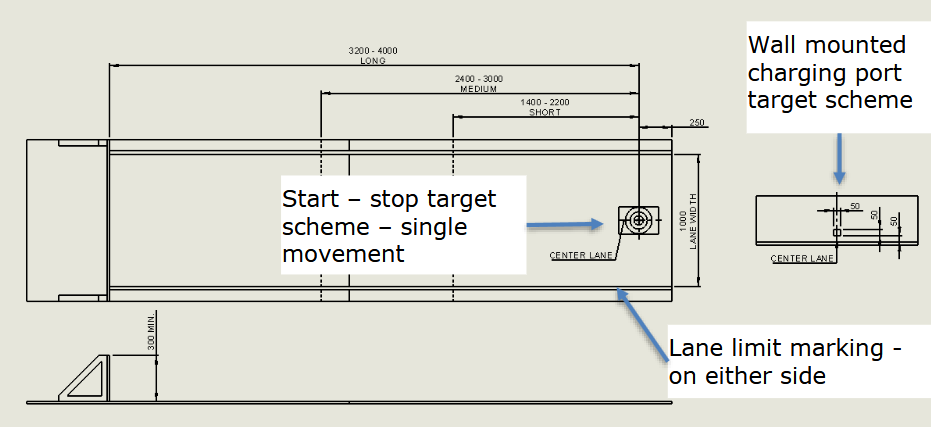
\includegraphics[width=0.8\textwidth]{extracted_images/image_4_2.png}\\
	\small\textbf{Figure 3:} Lane setup (dimensions in mm)
\end{center}
\subsubsection*{Measurement Tolerance}
$\pm$10mm using a single tape measure. Barrier positions vary in 50mm increments within each range.

\newpage\newgeometry{left=0.8in,right=0.8in,top=1in,bottom=0.6in}

\section{Product Design Specification}
Info is catered to the Foundation Group.
\subsection{Dimensional Requirements}
\begin{itemize}[itemsep=-0.7mm]
	\item Maximum working envelope: 400mm $\times$ 400mm $\times$ 400mm (including all components)
	\item Must maintain envelope compliance during all competition movements
\end{itemize}

\subsection{Required Components}
\begin{itemize}[itemsep=-0.7mm]
	
	\begin{figure}[H]
	\begin{minipage}{0.4\textwidth}	
	\centering\wm{0.8}{
	\item[\textbf{1.}] \textbf{Rear Datum Pointer}\\
		\textbf{-} Must remain vertical\\ 
		(pointing downward)\\
		\textbf{-} Max 6mm clearance from track surface\\
		\textbf{-} Determines device positioning
	}
	\end{minipage}\hspace{-2em}
	\begin{minipage}{0.7\textwidth}	
		\centering
		\begin{subfigure}[t]{0.45\textwidth}
			\centering
			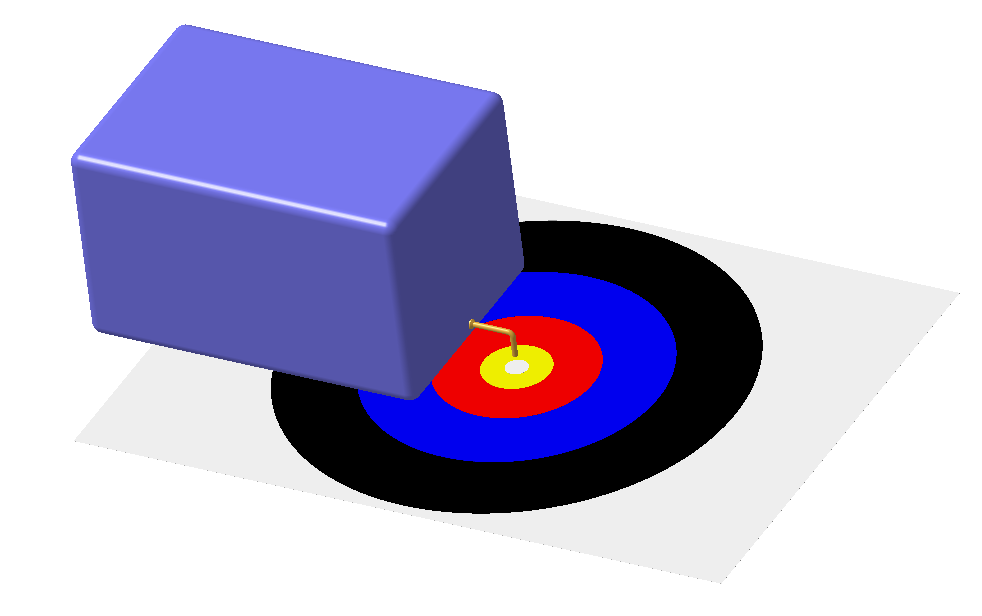
\includegraphics[width=0.7\textwidth,height=2.7cm]{extracted_images/image_10_2.png}
			\caption{Datum Pointer relative to the target}
			\label{fig:datumall}
		\end{subfigure}\hspace*{1em}
		\begin{subfigure}[t]{0.45\textwidth}
			\centering
			
\includegraphics[width=0.7\textwidth,height=2cm]{extracted_images/image_10_1.png}
			\caption{Datum Pointer (RS Components 397-4954)}
			\label{fig:datum}
		\end{subfigure}
		\caption{Datum Pointer Specification}
	\end{minipage}
	\end{figure}

	\begin{figure}[H]
	\begin{minipage}{0.4\textwidth}\vspace{-3em}
	\centering\wm{0.7}{\item[\textbf{2.}] \textbf{Single Front Plunger} (non-adjustable height for Foundation Group)\\\textbf{-} Max dimensions: 10mm $\times$ 10mm\\
	\textbf{-} Minimum protrusion: 10mm from device body when disengaged}
	\end{minipage}\hspace{-2em}
	\begin{minipage}{0.7\textwidth}			
		\centering
		\begin{subfigure}[t]{0.45\textwidth}
			\centering
			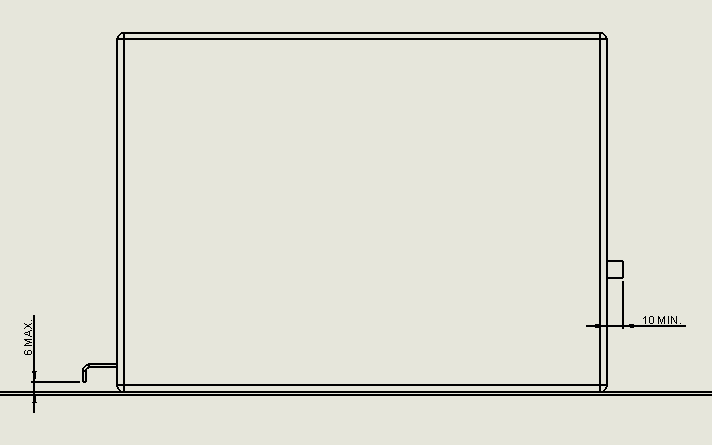
\includegraphics[width=0.7\textwidth,height=3cm]{extracted_images/image_11_2.png}
			\caption{Plunger Relative To The Datum}
			\label{fig:plungerall}
		\end{subfigure}\hspace{-1em}
		\begin{subfigure}[t]{0.5\textwidth}
			\centering
			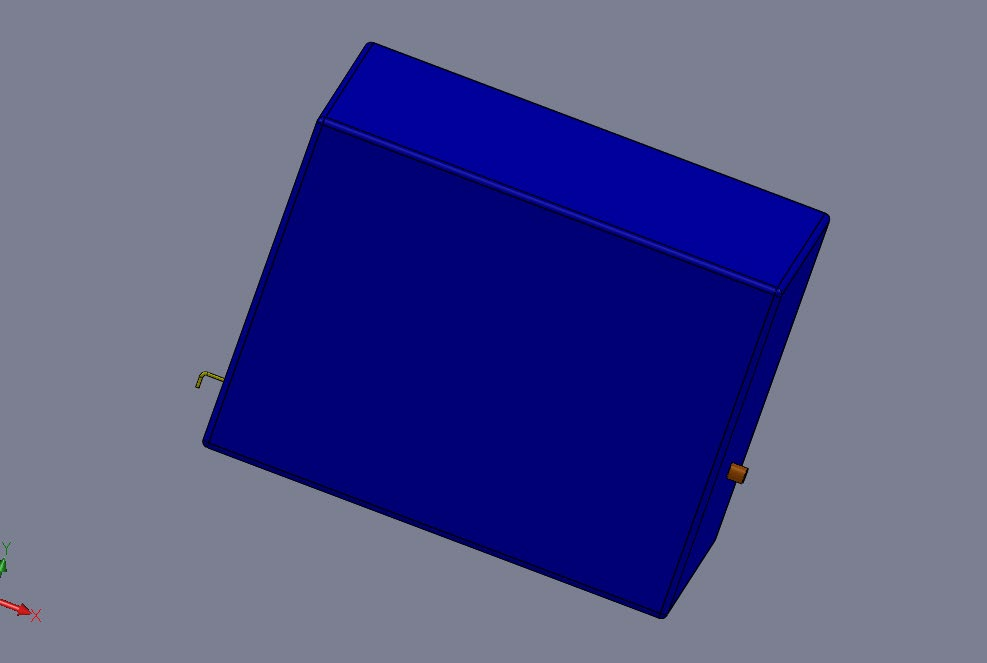
\includegraphics[width=0.7\textwidth,height=3cm]{extracted_images/image_11_1.png}
			\caption{Plunger (red thing)}
			\label{fig:plunger}
		\end{subfigure}
		\caption{Plunger Specification}
	\end{minipage}
	\end{figure}
\end{itemize}
\vspace*{-2em}
\subsection{Visual Indicators}
\begin{itemize}[noitemsep,topsep=0pt]
	\item Continuous green light during operation
	\item Red light + audible signal upon successful wall engagement
\end{itemize}
\subsection{Technical Restrictions}
\begin{itemize}[itemsep=-0.7mm,topsep=0pt]
	\item \textbf{No programmable circuitry} permitted (analog systems only)
	\item All repairs must be completed within allocated competition time
	\item Device must be fully self-contained (no external control)
\end{itemize}
\vspace{1em}\hrule\vspace{0.5em}
\subsection*{Key Differences from Advanced Category}
\begin{itemize}[itemsep=-0.7mm]
	\item No height adjustment capability required
	\item No programming or digital components allowed
	\item Simplified single-target operation
\end{itemize}


\newpage\newgeometry{left=0.8in,right=0.8in,top=1in,bottom=0.6in}
\section{Design Concepts}

\begin{minipage}{0.59\textwidth}
\subsection{Design Concept 1}
This was our initial concept idea, which had the advantage of being simple with minimal refinement. However, its main drawback was the high cost. While the model was accurate and met the specifications, its complexity and expensive manufacturing process made it difficult to produce.\\[8pt]
A major issue with this design is that high manufacturing costs can make large-scale production unfeasible. When a product is too costly to produce, it affects everything, from labor and machinery costs to production time, resulting in increased expenses and longer production timelines.
\end{minipage}\hfill
\begin{minipage}{0.4\textwidth}
\centering
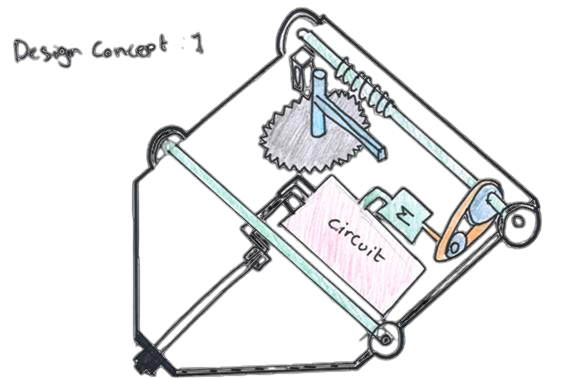
\includegraphics[width=1\textwidth]{images/image_6_2-Photoroom.png}
\captionof{figure}{Design Concept 1}
\end{minipage}\\[8pt]
The positives of this design is that it does meet the required specifications as it does fit the purpose of its role.\\[1em]
\begin{minipage}{0.59\textwidth}
	\subsection{Design Concept 2}
	This was our second design, which was simple and aesthetically pleasing. Its major strength was its ease of construction and compact size, which provided extra space for potential part exchanges or swaps. It was an adaptable design, but the main drawback was its susceptibility to breakages.\\[8pt]
	The negatives of this build are that it is prone to breakages, making it unreliable. This is crucial because during the testing phase, the design must pass to function correctly. If it is prone to breaking easily, it will reduce its longevity as materials deteriorate over time. The small size also means less room for improvements if needed.
\end{minipage}\hfill
\begin{minipage}{0.35\textwidth}
	\centering
	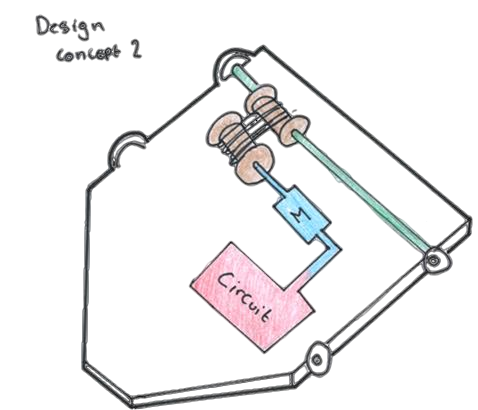
\includegraphics[width=0.95\textwidth]{images/image_7_2-Photoroom.png}
	\captionof{figure}{Design Concept 2}
\end{minipage}\\[4pt]
However, it is an aesthetic and versatile design, easy to swap parts if it breaks. The compactness is efficient for aerodynamics, and the lightness comes from the absence of bulky components.\\[1em]
\begin{minipage}{0.59\textwidth}
	\subsection{Design Concept 3}
	This was our final concept idea, which, like the first, had minimal refinement. Its major drawback was the cost, as it involved many unique moving parts. Although this design was durable and strong, it exceeded the budget outlined in the technical specifications.\\[8pt]
	The overall budget of this design was very high due to the numerous parts required, which increased manufacturing costs. There was also a lack of refinement, leading to inefficiencies in the design itself. The complexity of the build made assembly difficult, resulting in a higher likelihood of errors that could have been easily fixed with a simpler design. 
\end{minipage}\hfill
\begin{minipage}{0.4\textwidth}
	\centering
	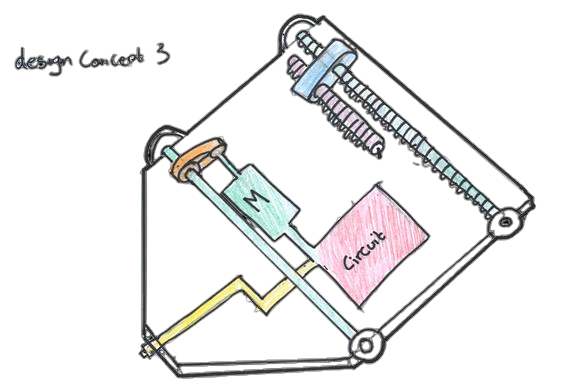
\includegraphics[width=1\textwidth]{images/image_8_2-Photoroom.png}
	\captionof{figure}{Design Concept 3}
\end{minipage}\\[8pt]
Despite this, it was a durable and strong design that could withstand impact and perform well.

\newpage
\section{Computer-Aided Design (CAD)}

\begin{minipage}{0.3\textwidth}
	\centering
	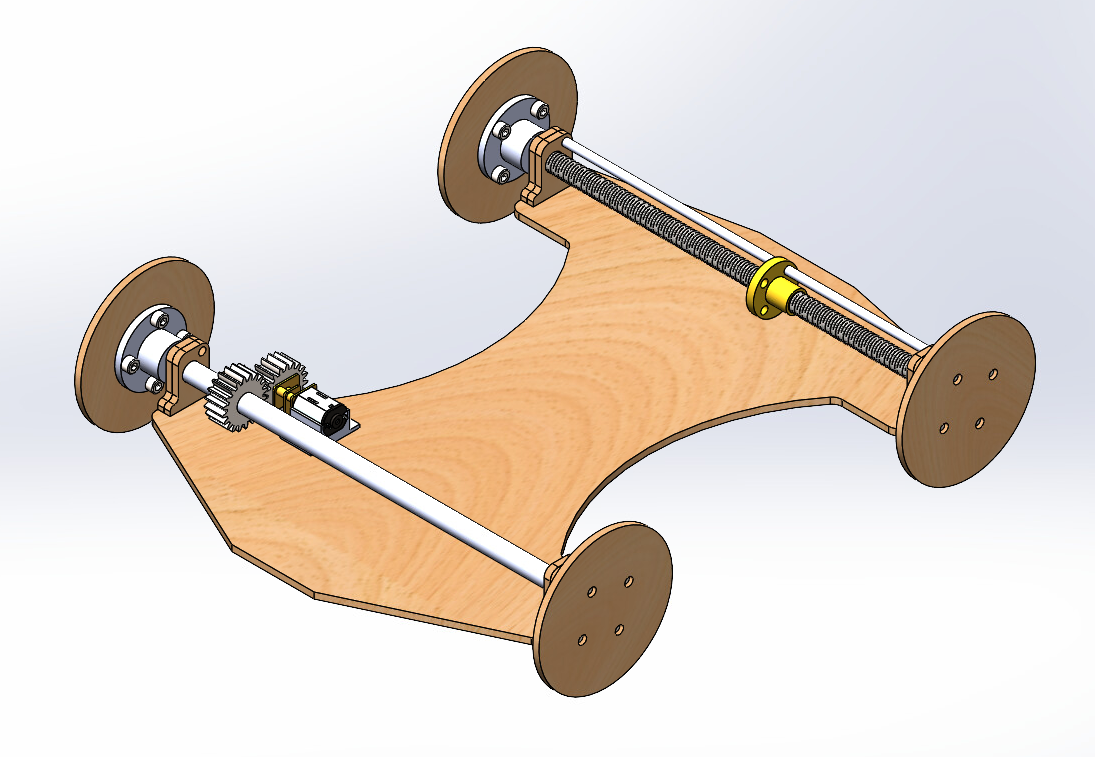
\includegraphics[width=1\textwidth]{extracted_images2/image(2).png}
	\captionof{figure}{Bottom Isometric View}
\end{minipage}\hfill
\begin{minipage}{0.3\textwidth}
	\centering
	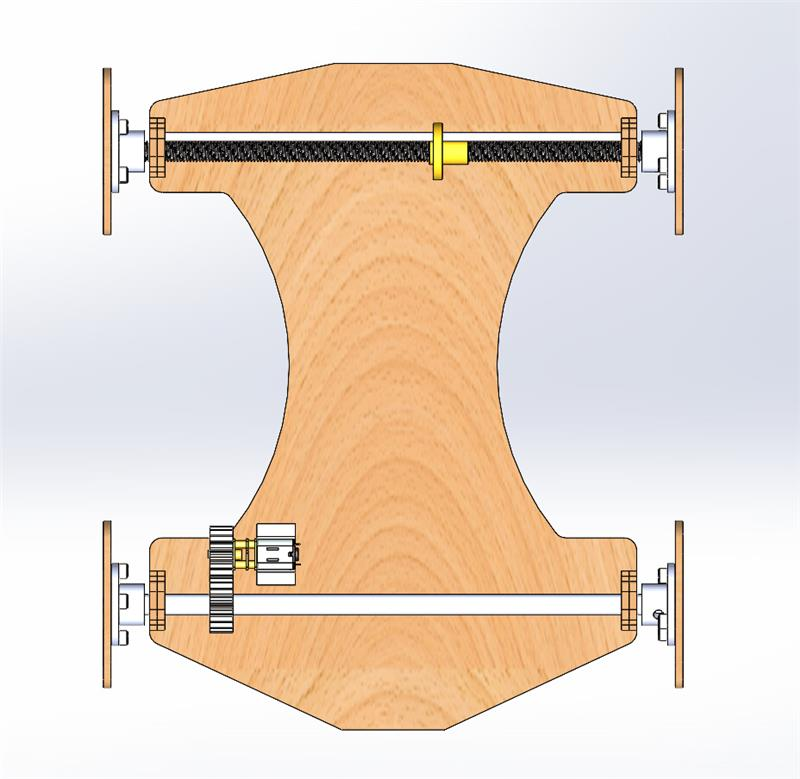
\includegraphics[width=0.7\textwidth]{extracted_images2/image.jpg}
	\captionof{figure}{Bottom Birds Eye View}
\end{minipage}\hfill
\begin{minipage}{0.3\textwidth}
	\centering
	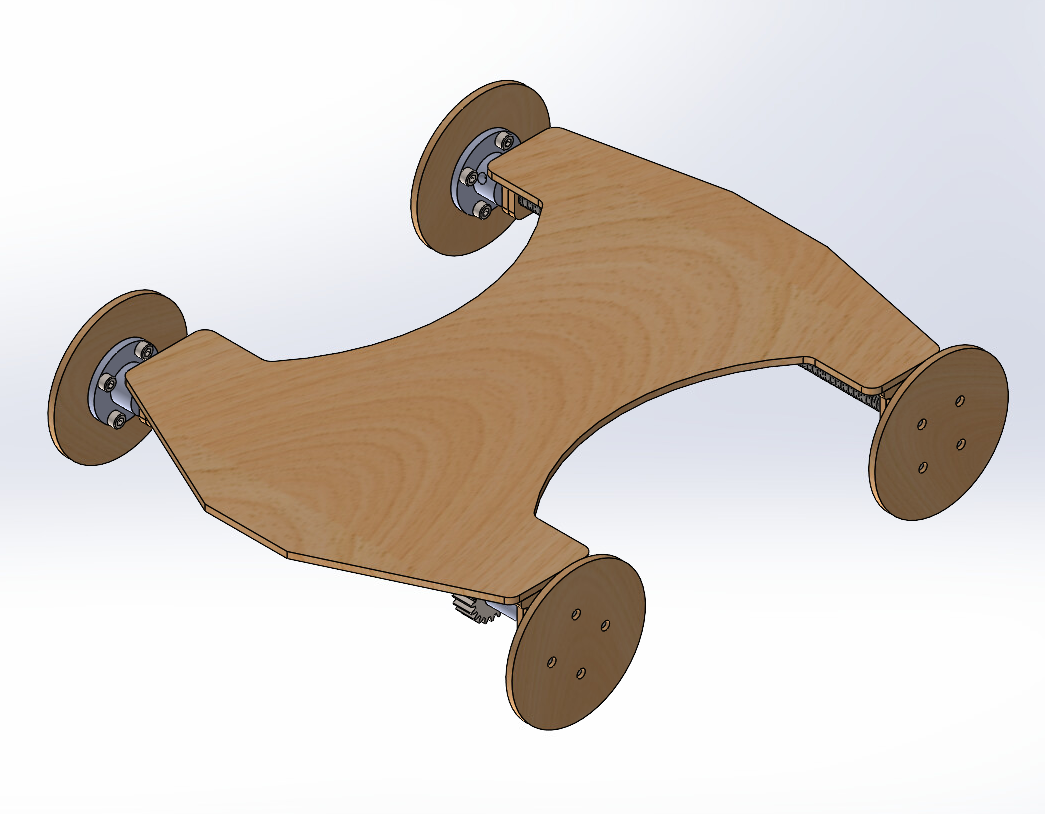
\includegraphics[width=0.9\textwidth]{extracted_images2/image(4).png}
	\captionof{figure}{Top Isometric View}
\end{minipage}\\[1em]
The images above illustrate various perspectives of the chassis design, modelled in SolidWorks. In the \textbf{Bottom Isometric View}, key components such as the chassis, shafts, and bearings are clearly visible. This mechanism forms the core structure that enables the vehicle's motion. A motor is attached to a threaded rod, which, when rotated, drives the rear wheels. Power is supplied via red and black wires connected to the motor, which interfaces with the main control circuit.\\[8pt]
Moving to the \textbf{Bottom Birds Eye View}, the image provides a clear representation of the base layout. This view emphasizes the arrangement of the front and rear shafts, both supported by mounts and bearings. The rear shaft is driven by the motor and connected to the rear wheels. The structural alignment ensures mechanical stability and efficient motion transfer from the motor to the wheels.\\[8pt]
Finally, the \textbf{Top Isometric View} offers an overall perspective of the design. This view was particularly useful for planning the placement of components and routing of wires. The breadboard was positioned on this side of the chassis, which was chosen as the front-facing side during the race. This decision was made due to the flat and spacious surface available, unlike the bottom section where the drive mechanism occupied most of the space. The ample area on this side allowed for secure placement of key components such as the battery pack, breadboard, and other electronic parts.
\vspace{0.8em}\hrule\vspace{0.2em}\noindent
\begin{figure}[H]
	\begin{minipage}{0.45\textwidth}
	\centering
	\begin{subfigure}[t]{0.45\textwidth}
		\centering
		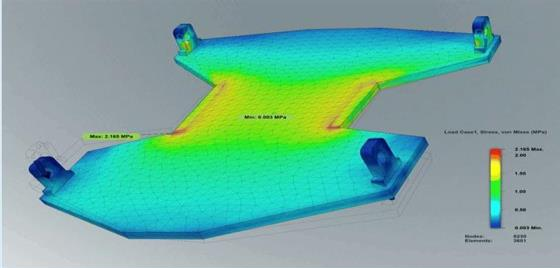
\includegraphics[width=1\textwidth,height=3cm]{images/feaone.png}
		\caption{FEA of the squared chassis design}
		\label{fig:fea_squared}
	\end{subfigure}%
	\hfill
	\begin{subfigure}[t]{0.45\textwidth}
		\centering
		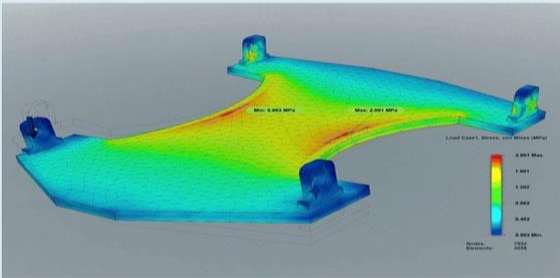
\includegraphics[width=1\textwidth,height=3cm]{images/featwo.png}
		\caption{FEA of the narrower chassis design}
		\label{fig:fea_narrow}
	\end{subfigure}
	\caption{Finite Element Analysis (FEA) comparing stress distributions between (a) the squared chassis and (b) the narrower chassis.}
	\label{fig:fea_comparison}
	\end{minipage}\hfill
	\begin{minipage}{0.5\textwidth}
		\subsection{Finite Element Analysis (FEA)}\large
		3D models of the vehicle’s base were developed using Fusion 360, and Finite Element Analysis (FEA) was carried out to assess structural stress distribution. Figure~\ref{fig:fea_comparison} compares two design variants: the squared chassis in Figure~\ref{fig:fea_squared} and the narrower, more streamlined version in Figure~\ref{fig:fea_narrow}.\\[8pt]
		The colour scale in each image represents stress intensity, where red and yellow indicate high stress, and green to blue indicate low stress regions.
	\end{minipage}		
\end{figure}\noindent
The squared design recorded a maximum stress of 2.165~MPa, while the narrower chassis showed a slightly reduced maximum of 2.001~MPa. Due to better stress distribution and reduced material usage, the narrower design was chosen for the final prototype.
\vspace{0.4em}\hrule\vspace{0.7em}\noindent
Using CAD software like SolidWorks or Fusion 360 allow for precise visualization of spatial requirements, ensuring that all electronic and mechanical components fit within the given constraints. CAD tools also enhance accuracy, reduce errors, and streamline the design-to-manufacture process. By simulating the design beforehand, potential issues can be resolved early, improving both cost-efficiency and production speed.

\newpage\newgeometry{left=0.7in,right=0.7in,top=1in,bottom=0.6in}
\section{Electronics}
Given the scope of this report and its intended audience, this section provides a overview of my electronics development journey---from initial concept to final implementation. Rather than a deep \textbf{technical} dive, it serves as a reflective summary, documenting key learnings, challenges, and methodological insights.\\[8pt]
At this academic level, the expectations for hands-on electronics proficiency were limited, and formal guidance was sparse. While I acknowledge that instructors prioritized foundational theory over practical support, this approach posed difficulties for beginners. Mastering the necessary electronics concepts---especially under time constraints---can take months, and the lack of structured mentorship made the process more daunting.\\[8pt]
The primary advice given was to use \textit{Tinkercad} for construction. While this tool has merits, I found it insufficient for my needs. Instead, I adopted a hybrid approach, blending theoretical understanding with targeted research to bridge knowledge gaps.
\vspace{-0.4em}
\subsection{Starting Structure}
\begin{minipage}{0.4\textwidth}
\begin{minipage}{1.6\textwidth}
My process started with building the core of the system:
\end{minipage}\\[8pt] 
\textbf{MOSFET-based H-bridge} using complementary P-channel and N-channel MOSFETs. At this stage, the focus was on creating two simple and clear signal inputs to control the motor:\\[8pt] 
\textbf{\texttt{DIR}} for direction (CW/CCW) and\\ \textbf{\texttt{PWR}} for enabling or disabling the motor.\\[8pt]
\begin{minipage}{1.6\textwidth}
 I approached the design with basic logic gates, using {AND} and {NOT} gates to process the inputs into the necessary control signals for the MOSFETs. 
\end{minipage}
\end{minipage}\hspace*{0.4em}
\begin{minipage}{0.4\textwidth}\vspace{-2em}
\begin{center}
\begin{tikzpicture}[
	scale=0.8,
	transform shape
	]
	\def\gap{3}	
	% PMOSFETs
	\node [pigfete,scale=0.8,name=fet1] at (0,2) {};
	\node [pigfete,scale=0.8,xscale=-1,name=fet2] at (\gap,2) {};
	% NMOSFETs
	\node [pigfete,scale=0.8,yscale=1,name=fet3] at (0,0) {};
	\node [pigfete,scale=0.8,yscale=1,xscale=-1,name=fet4] at (\gap,0) {};
	
	
	\draw (fet1.D) -- (fet3.S);
	\draw (fet2.D) -- (fet4.S);
	\coordinate (mottop) at ($(fet1.D)!0.5!(fet3.S)$);
	\coordinate (motbottom) at ($(fet2.D)!0.5!(fet4.S)$);
	\draw (mottop) to[short,*-*,current/distance=0.9,Telmech=M] (motbottom);

	
	\draw (fet1.S) -- ++(0,0.5) coordinate (vdd1);
	\draw (fet2.S) -- ++(0,0.5) coordinate (vdd2);

	\draw (vdd1) -- (vdd2) coordinate[midway] (mid1) (mid1) -- ++(0,0.5) node[above] {\normalsize \textbf{Vcc}} coordinate (mid1t); 
	
	\node[circle,color=black, fill=black, inner sep=0pt,minimum size=3pt] (b) at (mid1) {};
	
	\draw ($(mid1t)+(-0.3,0)$) -- ($(mid1t)-(-0.3,0)$);
	
	
	\draw (fet3.D) -- ++(0,-0.5) coordinate (gnd1);
	\draw (fet4.D) -- ++(0,-0.5) coordinate (gnd2);
	
	\draw (gnd1) -- (gnd2) coordinate[midway] (midpoint);
	\draw (midpoint) -- ++(0,-0.1) node[ground]{} coordinate[midway] (gnd);
	\node[below=0.7] at (gnd) {\footnotesize \textbf{GND}};
	\node[circle,color=black, fill=black, inner sep=0pt,minimum size=3pt] (b) at (midpoint) {};


%	\foreach \i in {fet1,fet3} {
%		\node at (\i.S) [left=-0.1] {\tiny\(S\)};
%		\node at (\i.D) [left=-0.1] {\tiny\(D\)};
%		\node at (\i.G) [left=-0.1] {\tiny\(G\)};
%	}
%
%	\foreach \i in {fet2,fet4} {
%		\node at (\i.S) [right=-0.1] {\tiny\(S\)};
%		\node at (\i.D) [right=-0.1] {\tiny\(D\)};
%		\node at (\i.G) [right=-0.1] {\tiny\(G\)};
%	}
	\node at (fet1) [right=0.3cm] {\small\(P_1\)};
	\node at (fet2) [left=0.3cm] {\small\(P_2\)};
	\node at (fet3) [right=0.3cm] {\small\(N_1\)};
	\node at (fet4) [left=0.3cm] {\small\(N_2\)};
	
	
	\def\a{0.4}
	\def\b{0}
	
	\def\sigx{1}
	
	\def\left{-0.4}
	\def\lefto{-0.4}
	
	\def\leftot{\lefto*2}

	
	
	\node[ieeestd not port, anchor=in, scale=0.5] (not1) at ($(fet1.G) + (-1,0)$) {};
	\node[ieeestd not port, anchor=in, scale=-0.5] (not2) at ($(fet2.G) + (1,0)$) {};
		
	\node[ieeestd and port, anchor=in 1, scale=0.5] (and1) at (-4,1.4-\b) {};	
	\node[ieeestd and port, anchor=in 1, scale=0.5] (and2) at (-4,0-\a) {};
	
	\coordinate (not0pos) at ($(and1.in 1) + (-1,1)$);
	\node[ieeestd not port, anchor=out, scale=0.5] (not0) at (not0pos) {};	
	
	\draw (not0.out) -| ($(and1.in 1) + (\left,0)$)-- (and1.in 1);
		
	\coordinate (not01pos) at ($(and2.in 2) + (-1,0)$);
	\node[ieeestd not port, anchor=out, scale=0.5] (not01) at (not01pos) {};	

	\draw (not01.out) -- (and2.in 2);
	
	\coordinate (midand) at ($(and2.in 1)!0.5!(and1.in 2)+ (-2.4,0)$);		
	\draw ($(midand)+(-\sigx,0)$) coordinate (dir) -- (midand) node[circ] {};
	\draw (midand) |- (and1.in 2);	
	\draw (midand) |- (not01.in);
	
	\draw ($(and1.in 1)+(\left,0)$) |- (and2.in 1);	
	
	\draw (and1.out) -| ($(fet3.G)+(\leftot,0)$) -- (fet3.G);
	\draw ($(fet3.G)+(\leftot,0)$) -- ($(fet3.G)+(\leftot,-2.7)$) -| ($(not2.in)-(\lefto,0)$) -- (not2.in);	

	\draw (and2.out) -| ($(not1.in)+(\lefto,0)$) -- (not1.in);	
	
	\node[circ] at ($(fet3.G)+(\leftot,0)$) {};
	
	\draw ($(and2.out-|not1.in)+(\lefto,0)$) --($(and2.out-|not1.in)+(\lefto,-2.7)$) -| ($(fet4.G)-(\lefto,0)$) -- (fet4.G);
	
	\node[circ] at ($(and2.out-|not1.in)+(\lefto,0)$) {};

	\node[circ] at ($(and1.in 1)+(\left,0)$) {};


	\draw (not1.out) -- (fet1.G);
	\draw (not2.out) -- (fet2.G);

	
	\draw (not0.in) --++(-\sigx*1.5,0) coordinate (pwr);
	
	\node[label={[font=\large]120:\textbf{\texttt{PWR}}}, draw, circle, fill=white, draw=black, scale=0.5,thick] at (pwr) {};

	\node[label={[font=\large]120:\textbf{\texttt{DIR}}}, draw, circle, fill=white, draw=black, scale=0.5,thick] at (dir) {};
			
	\end{tikzpicture}
\end{center}
\end{minipage}\\[8pt]
The logic was straightforward yet crucial, as it needed to handle some key responsibilities:\\[5pt]
\hspace*{-1em}
\begin{minipage}{0.53\textwidth}
	\textbf{Power Disable Mode (\texttt{PWR = 1}):} 
	When the power signal is high, the system disables motor drive, allowing it to coast to a stop.
	\begin{itemize}[itemsep=-1mm]
		\item \code{1} : Activates both high-side MOSFETs ($P_1$, $P_2$)
		\item \code{0} : Direction control (\texttt{DIR}) becomes active
	\end{itemize}	
\end{minipage}\hspace{1em}
\begin{minipage}{0.5\textwidth}
	\textbf{Direction Control Mode (\texttt{PWR = 0}):} 
	When power signal is disabled, the direction signal determines the active MOSFET pairs (a bit awkward, I know):
	\begin{itemize}[itemsep=-1mm]
		\item \code{1} : Reverse direction ($P_2$ and $N_1$ activated)
		\item \code{0} : Forward direction ($P_1$ and $N_2$ activated)
	\end{itemize}
\end{minipage}\\[8pt]
This initial switching matrix became the backbone of the system, and everything I built afterward had to integrate seamlessly with this simple but essential layer. I made sure to carefully test and validate the gate network, ensuring it was stable and reliable before moving on to more complex features. Ultimately, the success of the entire system depended on the reliability of this basic setup.
\vspace{-0.4em}
\subsection{Prioritizing Pause Logic}
With the H-bridge logic in place, the next challenge was to implement a method to {pause the motor} for a fixed duration, triggered via physical contact. I decided to use a \textbf{555 timer} with a push-button trigger. The timer was configured to generate a $\sim$15-second HIGH pulse upon activation, with the configuration $$1.1 \times 470\ \mu{F} \times 27\ {k}\Omega\approx 15s$$
The HIGH output from the timer was was essentially my \texttt{PWR} signal. This way, while the timer was active, \texttt{1}, the motor would {coast/stop}. Once the timer expired, \texttt{0}, the motor would resume operation. By this point, the directional control, \texttt{DIR}, was fixed, and I planned to tackle that aspect later, after establishing a reliable pause-reset flow.

\subsection{Direction Logic}
\subsubsection{Button-Based Reversal}
With the timer working, I wanted to make the motor {switch direction} after each cycle. My first idea was to {reuse the same push-button} that triggered the 555 timer to also reverse the direction. I designed a separate logic circuit using transistors, capacitors, and button presses to toggle the signal. It worked perfectly in isolation. However, when I tried to integrate it into the 555 setup, things didn’t go as planned. The reversal circuit and the timer had different assumptions about how the button behaved, leading to conflicting logic and erratic behavior. I ultimately abandoned this approach.

\subsubsection{Relay Logic}
After abandoning the button-based method, I came up with a better idea: to use the {555’s own output pulse} to handle direction switching. This would separate the trigger from the direction logic, making the system more modular.\\[8pt]
In {CircuitJS}, I built a setup using a \textbf{relay} that flipped the direction signal each time the 555 pulse occurred. It worked as expected-the relay acted like a physical toggle, and I used invisible labels to manage virtual connections and logic states.\\[8pt]
However, when I tried to replicate this in {Tinkercad}, it didn’t work. Tinkercad couldn’t support the internal relay wiring or virtual labels I had used in the simulation, so I had to rethink the approach. After much trial and error, I found it difficult to make the setup work in that platform and generally in a physical sense as well--it just felt bulky and inefficient. I needed something cleaner and more logical, not forced.

\subsubsection{T Flip-Flop}
Frustrated, I turned to an online forum. A helpful suggestion came through: {use a T flip-flop.}\\
This turned out to be exactly what I needed. A \textbf{T flip-flop} toggles its state on every clock pulse-in my case, the falling edge of the 555 timer output. This solution completely decoupled the direction logic from the button and worked perfectly both in theory and in practice.\\[3pt]
I set it up so that:
\begin{itemize}[itemsep=-1mm]
	\item The {555 timer} would disable the motor for 15 seconds.
	\item When the pulse ended, the falling edge would clock the {T flip-flop}, toggling the output(s) in which in turn would then feed into the direction signals of the relevant AND gate.
\end{itemize}
This setup was stable, minimal, and, most importantly, felt right.

\subsection{Breadboarding}
Moving from simulation to real hardware brought its own set of challenges.
\begin{itemize}[itemsep=0mm]
	\item First, the {T flip-flop} (actually implemented using a J-K flip-flop with both J and K set high to mimic T flip-flop behavior, and using {PRE} and {CLR} as reset) behaved unpredictably. It turned out the trigger was {floating}, and I hadn’t added pull-down resistors (new to me at the time). Simulations hadn’t shown this, but adding the resistors fixed the issue.
	\item I also realized the 555’s button needed debouncing. Since the 555 timer was in monostable mode, if the button was pressed longer than the pulse duration, it wouldn’t change state as expected. To solve this, I added two 10kΩ resistors and a 0.1µF capacitor with the button. This ensured the 555 timer was triggered only once per button press, even if the button was held down longer than the pulse duration.
	\item By now, I had long since moved beyond Tinkercad. It couldn’t simulate well and too many things didn’t behave as they did in the real world. I felt competent enough to resolve problems if and when there were any at this point.
\end{itemize}
\newpage
\subsection{Final Behavior -- What It Actually Does}
Here’s what the final circuit accomplishes:
\begin{itemize}[itemsep=-1mm]
	\item Pressing a {button} triggers a 15-second pulse via a {555 timer}.
	\item While the pulse is active, the {inverted output} disables the motor.
	\item When the timer ends, the {T flip-flop toggles} the direction.
	\item Logic gates maintain signal integrity and enforce state rules.
	\item A {limit switch} cuts the circuit entirely if triggered (end of race), providing a safety cutoff.
\end{itemize}
Additional tasks such as cleaning signals, filtering, and ensuring smooth overall behavior were then implemented, along with essential components like the buzzer, fuse box, and other relevant compliances, all placed in their respective places.\\[8pt]
While I had intended to discuss the PCB creation, that step was never completed---thanks to the university's machine breaking down just before I could proceed.

\subsection{Circuit Diagrams and Breadboard Setup}
The underlying main circuit schematic is shown below:\\
\hspace*{-2em}
\begin{minipage}{0.4\textwidth}
	\centering
	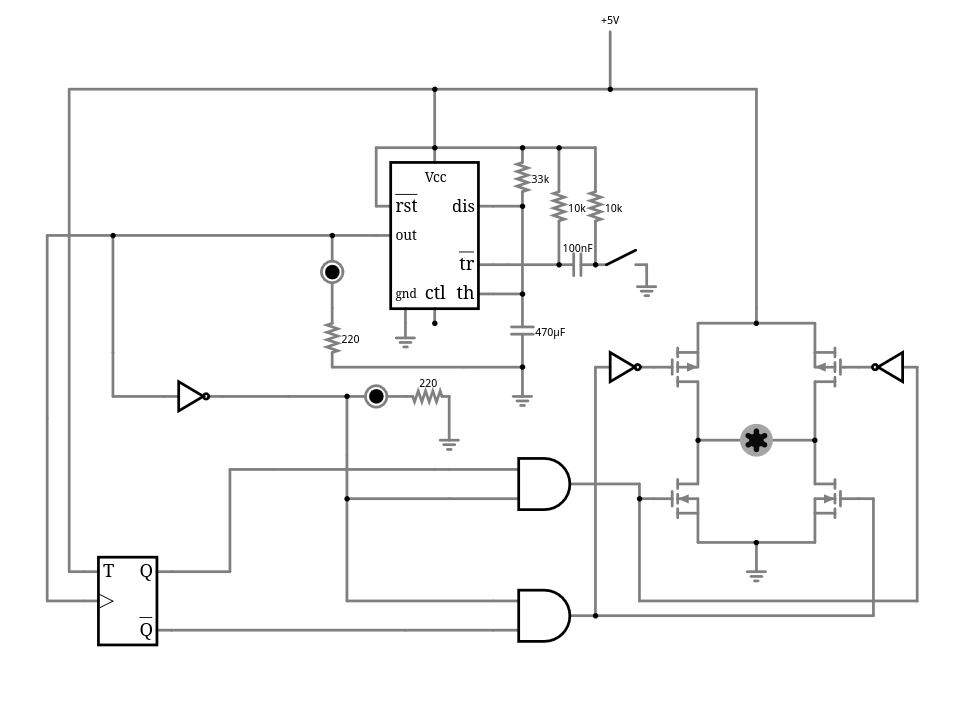
\includegraphics[width=1\textwidth]{images/swappy-20250406-185116.png}
	\captionof{figure}{Main Circuit Schematic}
\end{minipage}\hspace{1em}
\begin{minipage}{0.5\textwidth}
	\centering
	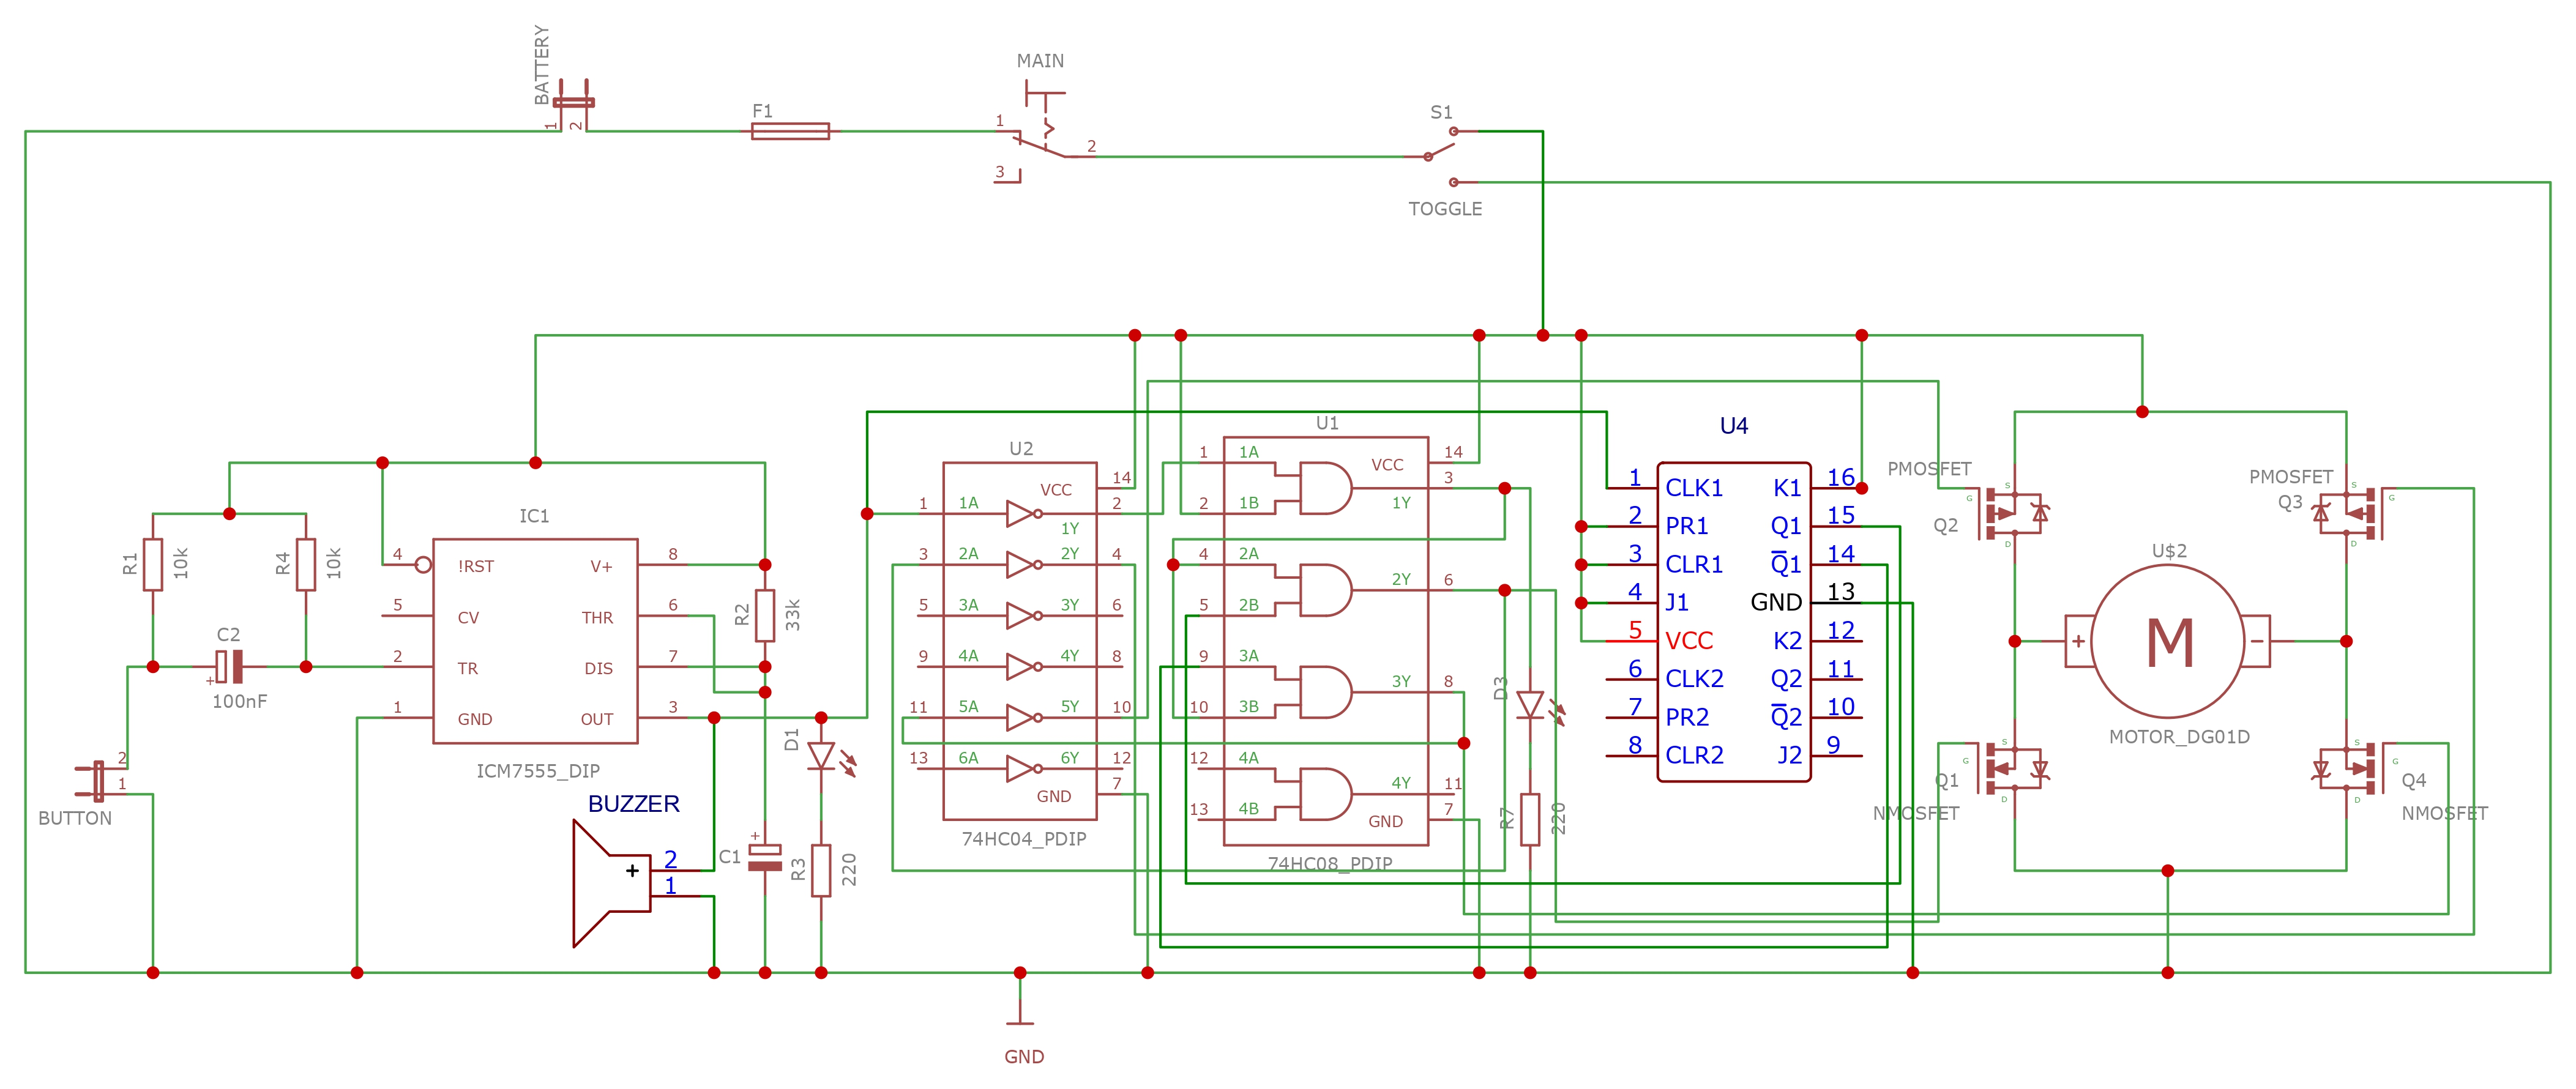
\includegraphics[width=1.3\textwidth]{images/Schematic_SAKARIYEPCB.sch_2025-04-06_page-0001.jpg}
	\captionof{figure}{Breadboard Schematic}
\end{minipage}\\
\begin{figure}[H]
	\centering
	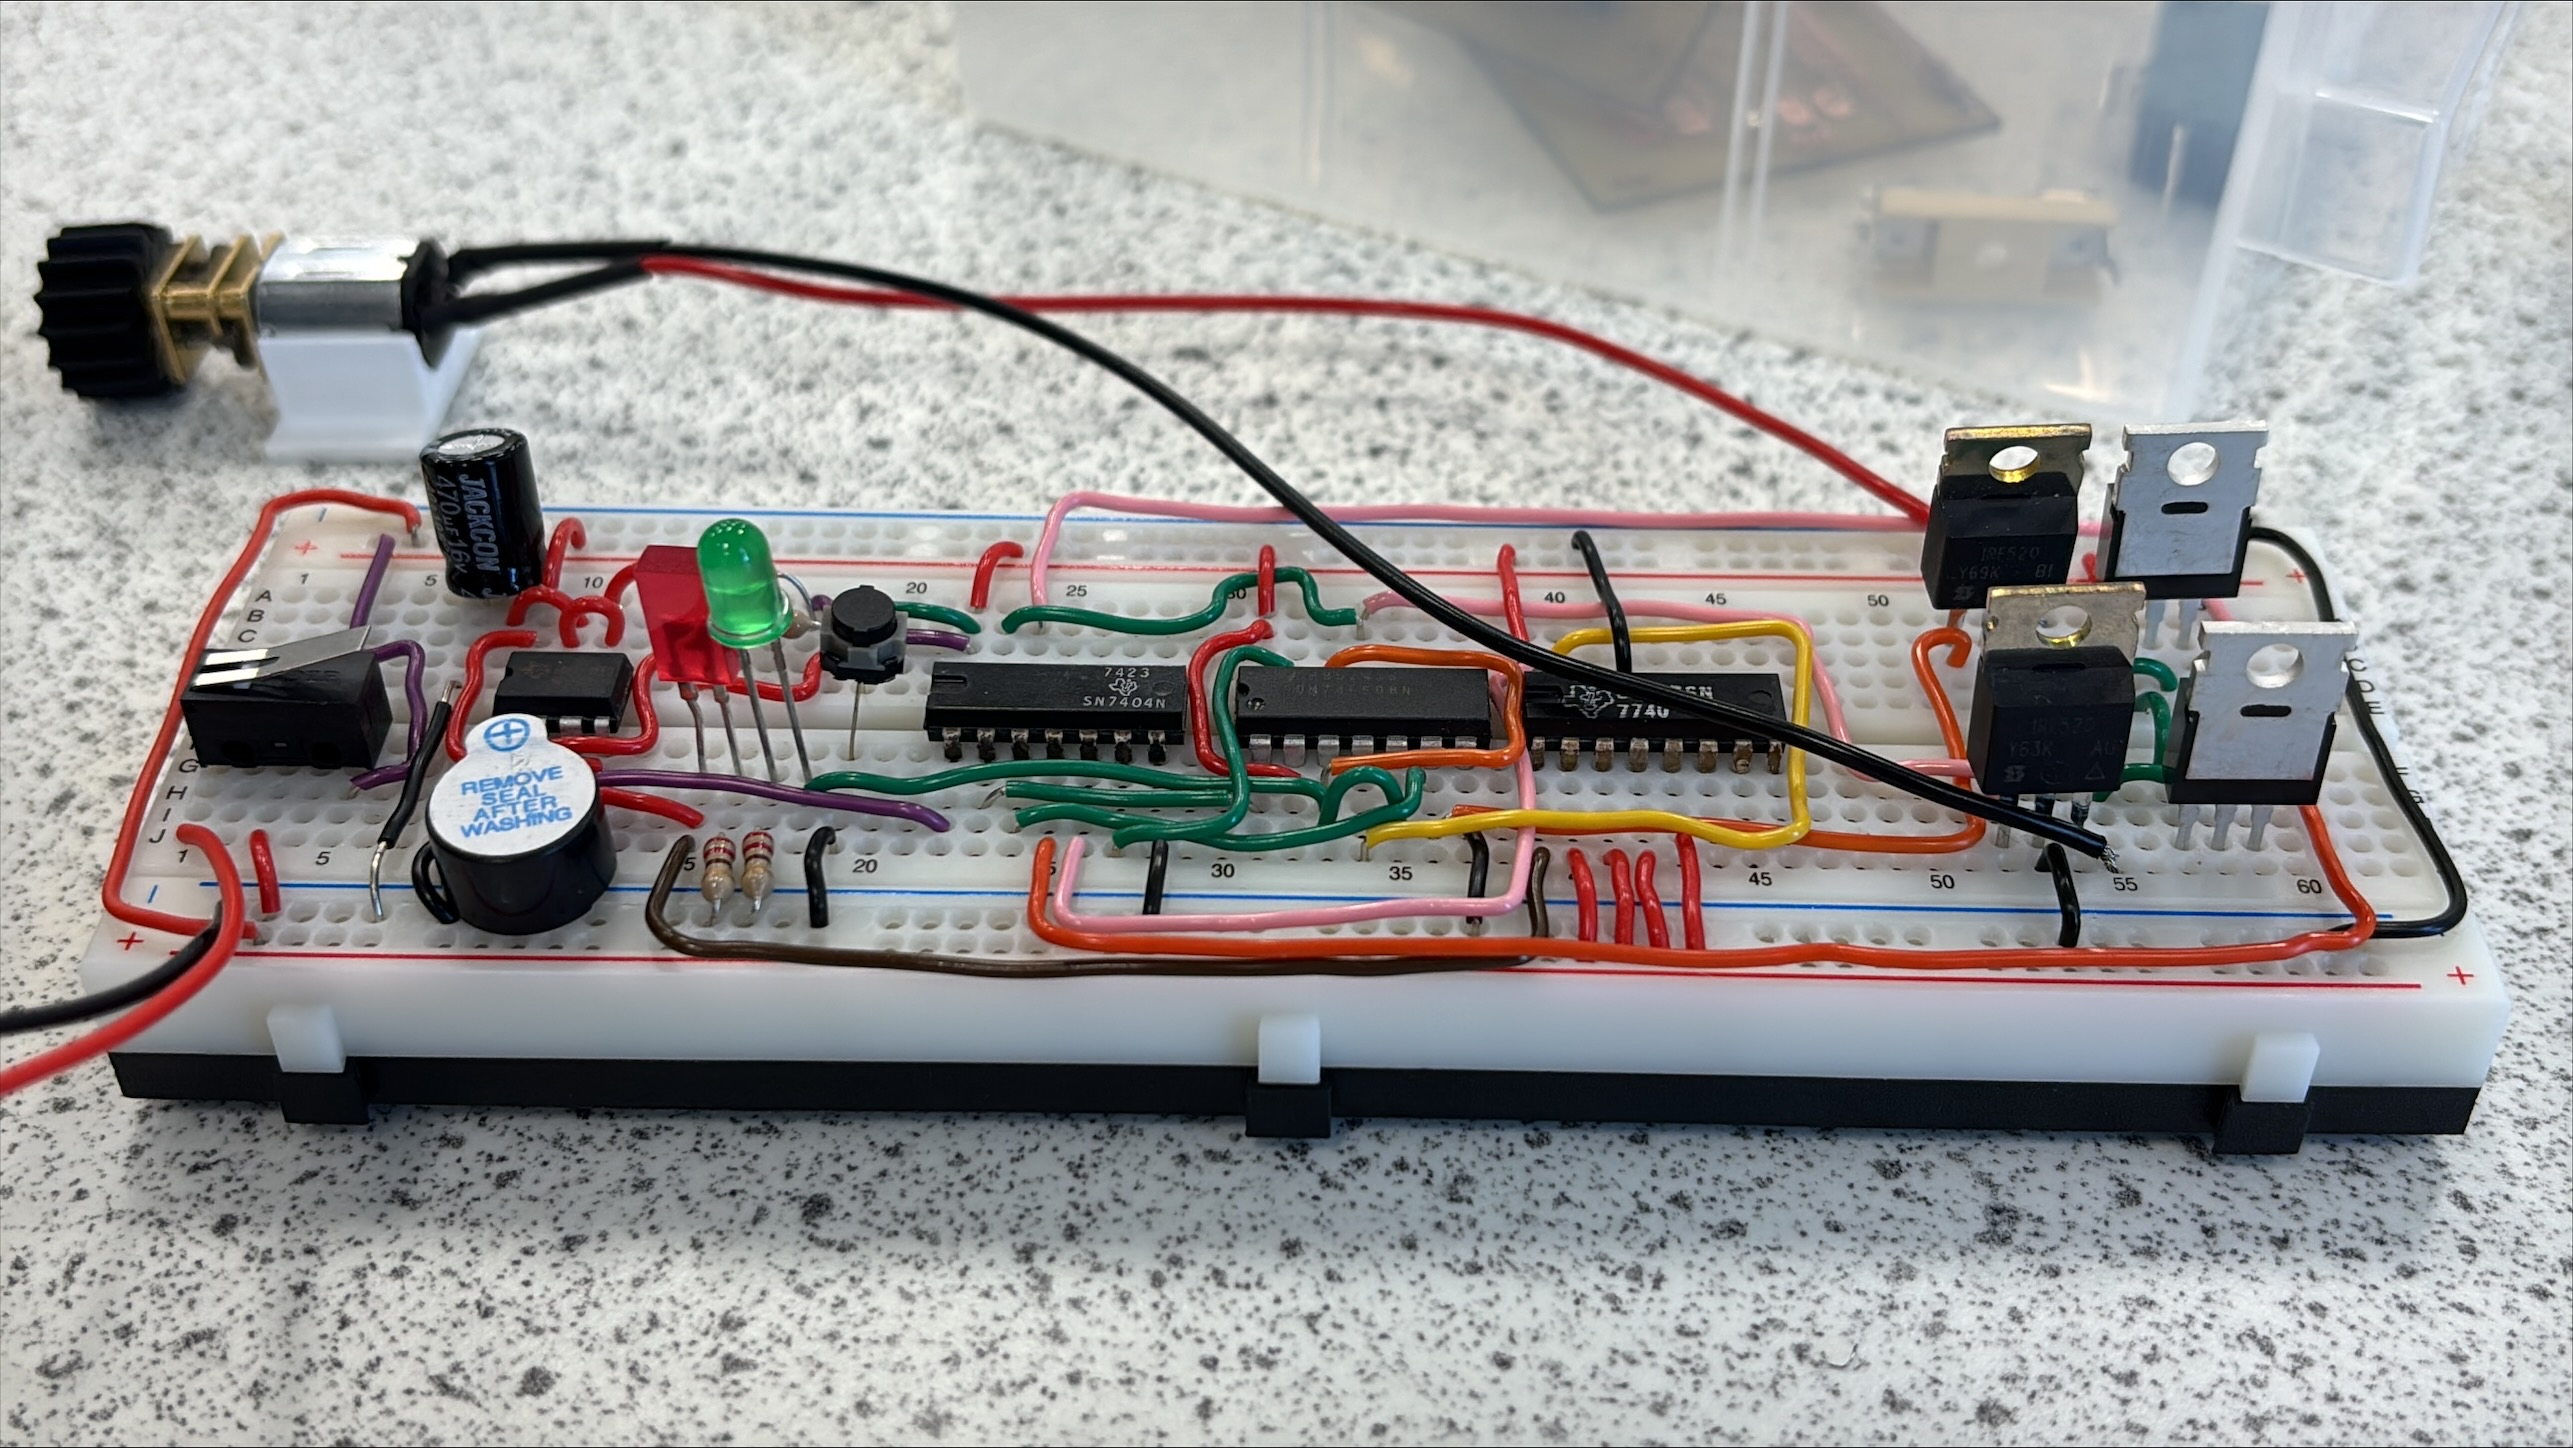
\includegraphics[width=0.6\textwidth]{images/Image(2).jpg}
	\caption{Breadboard Setup}
\end{figure}\noindent
These diagrams and setups were/are subject to change as the project progressed. They are included here to illustrate the foundational premise of the design. You may notice discrepancies, such as the RC debounce, fuse box, limit-switch, and other minor details, please note these are things refined and adjusted throughout the process.

\newpage
\phantomsection
\refstepcounter{section}
\addcontentsline{toc}{section}{\thesection\quad Bill Of Materials (BOM)}
\refstepcounter{subsection}
\addcontentsline{toc}{subsection}{\thesubsection\quad Mechanics}
\refstepcounter{subsection}
\addcontentsline{toc}{subsection}{\thesubsection\quad Electronics}

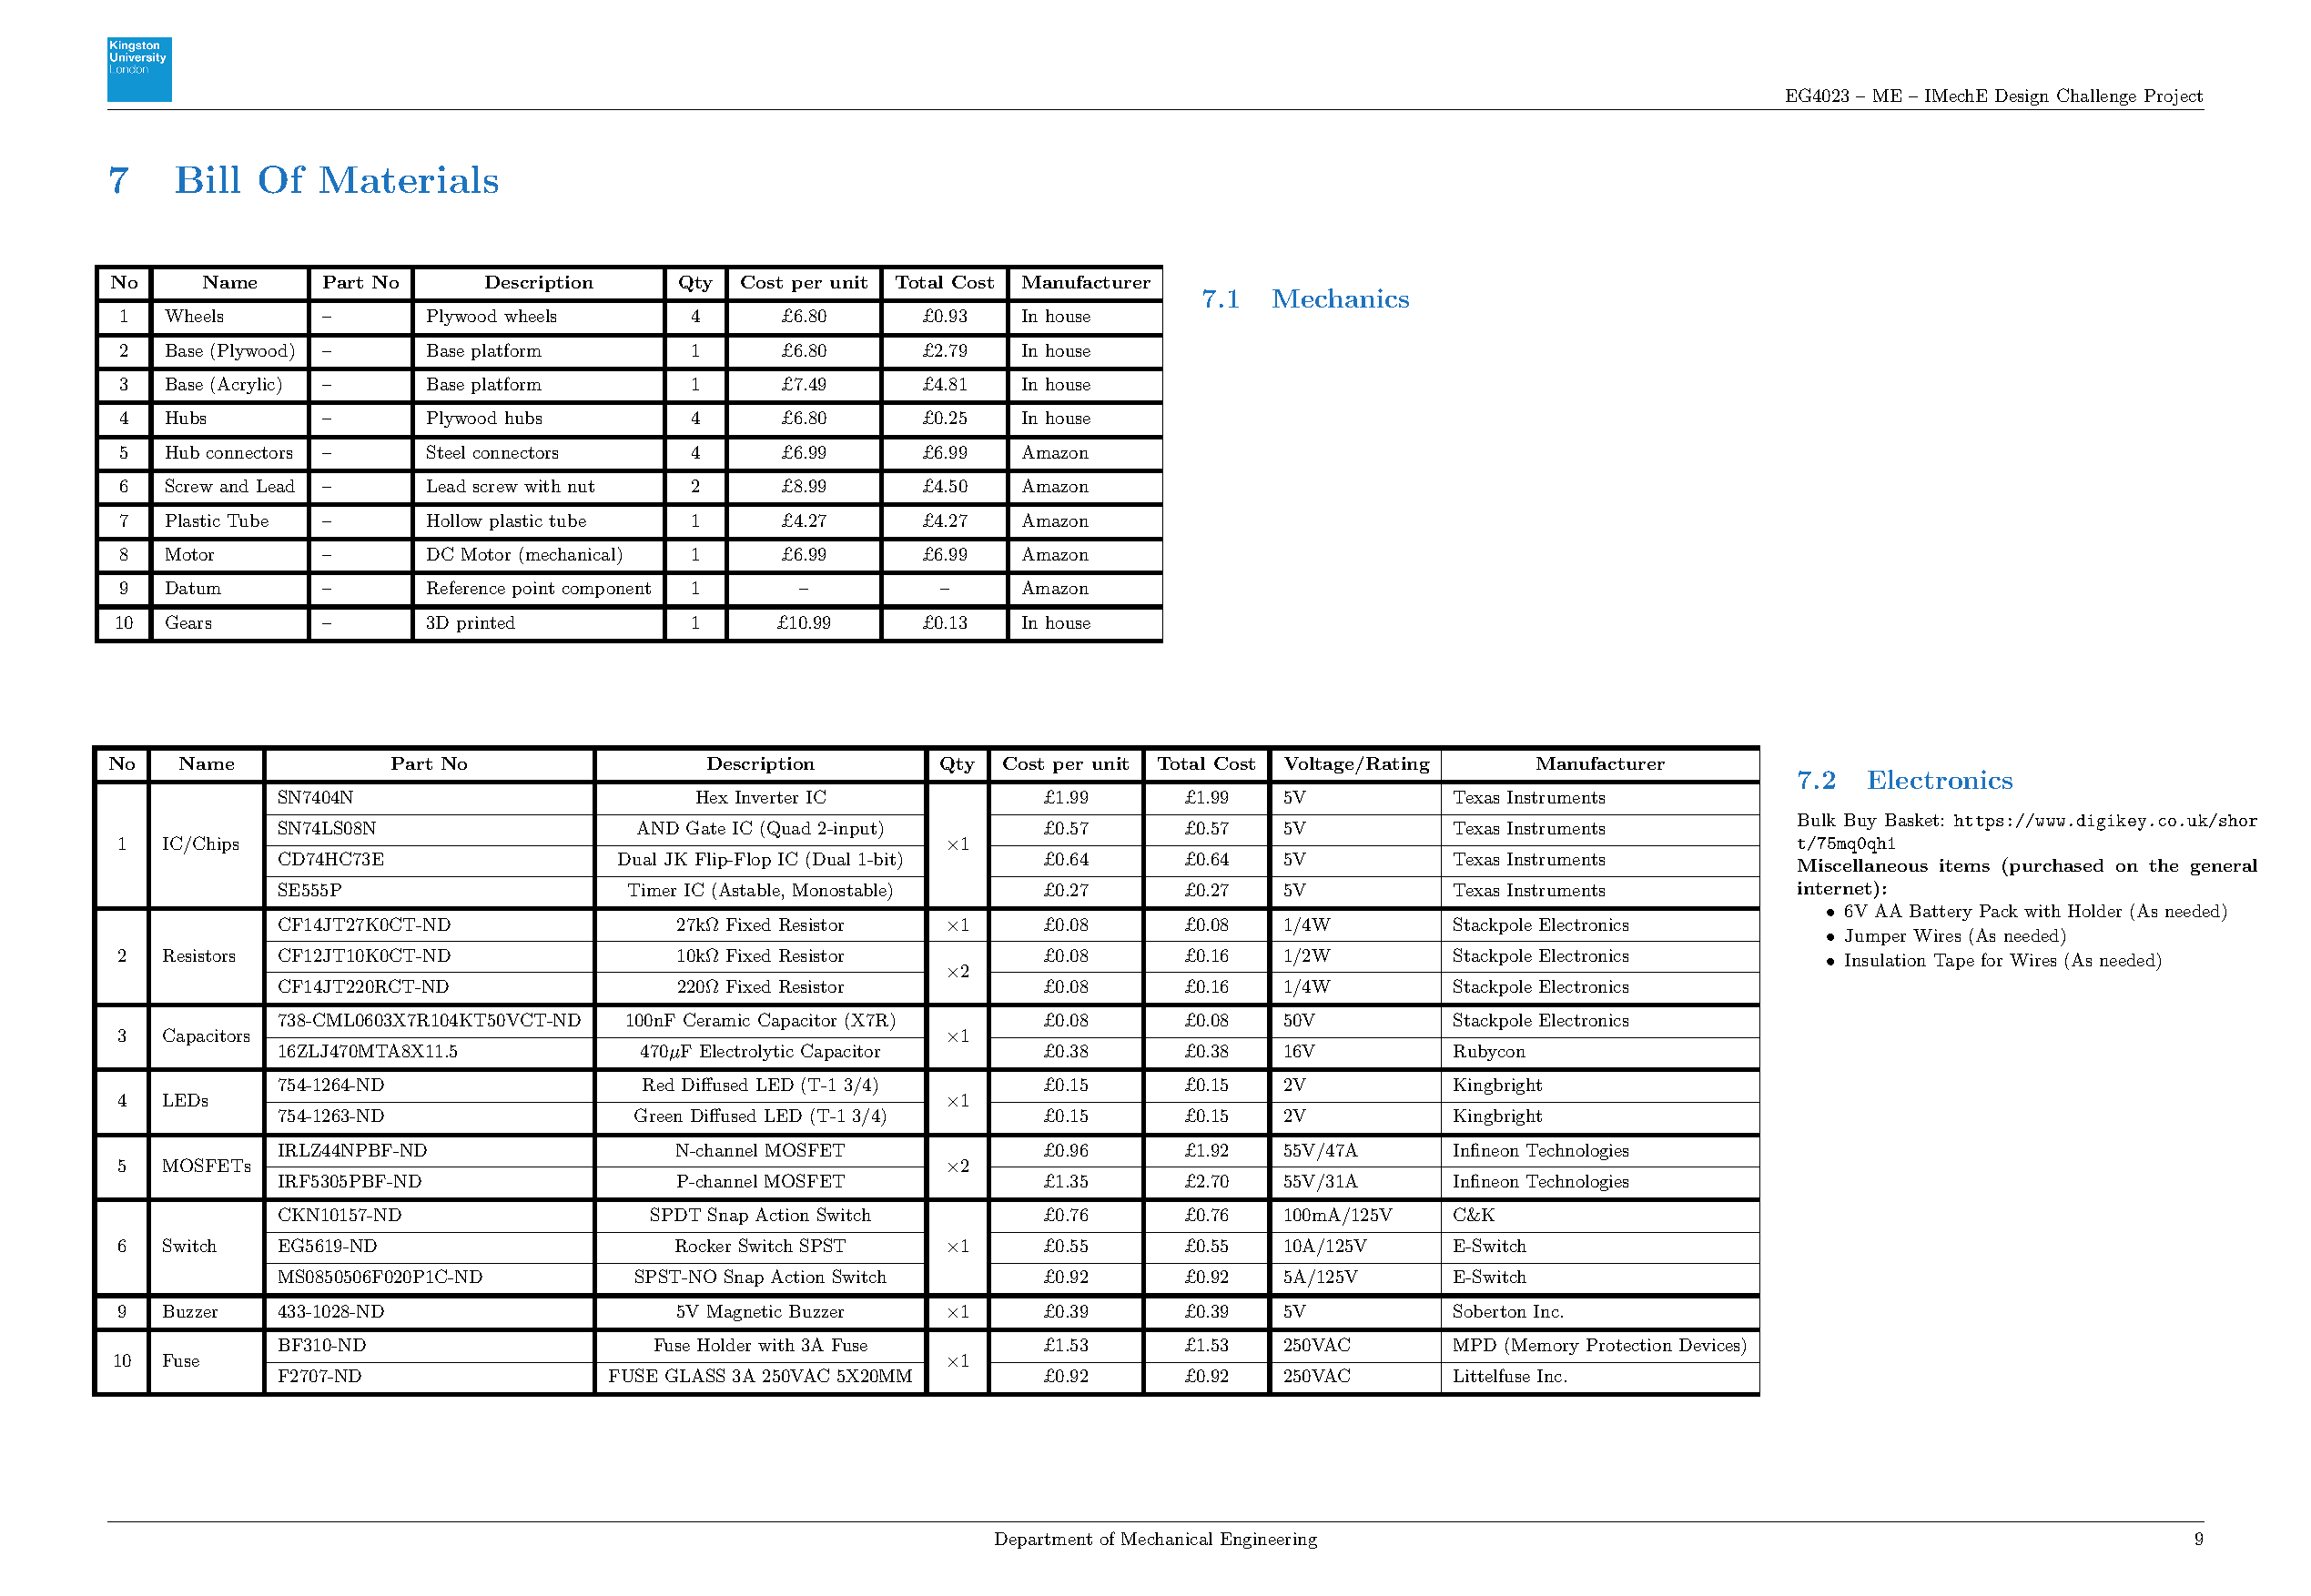
\includepdf[pages=-,landscape,fitpaper]{bom/bom.pdf}

\restoregeometry\newgeometry{left=0.8in,right=0.8in,top=1.1in,bottom=0.69in}

\section{Manufacturing Process}

\begin{itemize}
	\item \textbf{Stage 1:} The initial part of the manufacturing process was sourcing the raw materials needed and ordering any parts. We were able to source the plywood sheet, plastic axle, and all electrical components in-house. The screw thread rod and flange connectors were purchased online. Subsequently, we sourced acrylic in-house.
	
	\item \textbf{Stage 2:} We made the chassis next, which was laser cut from 3mm plywood to size. The wheels and hubs were also laser cut from the same plywood to save material and time.
	
	\item \textbf{Stage 3:} The next part was to glue the hubs to the chassis using Gorilla Glue Super Glue. During the drying time, the holes for the wheels to mount onto the connectors were drilled using a hand drill. These were then fitted using nuts and bolts.
	
	\item \textbf{Stage 4:} The screw thread rod was then cut down to size using a junior hacksaw and filed to clean up the roughness of the edge. The plastic axle was also cut down to size using a hacksaw and then sanded.
	
	\item \textbf{Stage 5:} The gears were 3D printed and mounted onto the motor and plastic axle by heating them up with a heat gun, melting them, and allowing them to dry onto the components, creating a sealed bond. The motor housing was 3D printed as well and glued to the chassis using a hot glue gun.
	
	\item \textbf{Stage 6:} The screw thread rod and plastic axle were then fitted to the chassis and hubs, secured onto the connectors. We now had a rolling vehicle.
	
	\item \textbf{Stage 7:} During these previous stages, the electronics had been in the works and were now ready to be laid out on the breadboard. The initial breadboard had loose wires, so a new, neater one was created.
	
	\item \textbf{Stage 8:} The plunger was fitted to a wooden block by creating a pilot hole for the thread to screw into and then glued onto the rear of the vehicle using a hot glue gun. The switch for the front of the car to stop it when it hits the wall and the switch to end the journey were mounted using a hot glue gun.
	
	\item \textbf{Stage 9:} The electrical components were fitted to the car and wires connected and held with electrical tape; we now had a functioning car.
	
	\item \textbf{Stage 10:} We decided to change the design and added a new acrylic chassis which was laser cut from the previous design and glued to the plywood one with Gorilla Glue Super Glue.
\end{itemize}
\vspace*{0.2em}
\section{Testing \& Improvements}

\subsection{Prototype 1:}
Although our first prototype complied with all specifications, it had certain drawbacks that ultimately affected the overall performance, durability, and accuracy of the vehicle. After considered analysis, we decided to change and redesign certain parts to eliminate these problems. Design for Manufacturability (DFM) was a key area we focused on, changing materials and components used.

\subsubsection{Chassis:}
The chassis was made from 3mm plywood and laser cut to size. Plywood is lightweight and a relatively inexpensive material, so we thought it would be a good option. However, upon building the car, we discovered the plywood was ever so slightly warped. When testing, we found the car would steer off to one side, meaning it would not hit the required target on the wall. This was due to a multitude of reasons, including wheel alignment, uneven weight distribution, different rolling resistance, and axle misalignment. This was an easy fix; the solution was to change the material from plywood to acrylic, eliminating any possibility of natural wood defects.

\subsubsection{Wheel Hub:}
The wheel hubs were also made from 3mm plywood and laser cut to size. The issue occurred with the mounting onto the chassis. We measured it by hand and glued it to the underside of the chassis. This presented issues with alignment as we relied on the accuracy of manual human precision and judgment. Even after careful measurement, the hubs were not perfectly aligned on the chassis, causing problems similar to the warping issue. Using just glue as the joining method has its drawbacks as that area will now be weak under stress, only providing strength in tension and not in shear or peel. The surface preparation and conditions have a direct impact on the placement of these hubs, especially since the chassis was warped. This didn't offer any reusability or adjustability, meaning that once glued, we couldn't change or undo the bond. Over time, under constant load, the glue joints can deform slowly, reducing the accuracy of direction. Our solution to this problem was to design a new 3D printed wheel hub that slotted into the chassis from a laser cut-out section. This is held in place with a dowel-type joint and means no glue, manual human accuracy, or measuring is needed. Simply slot the hub into the chassis, and it's perfectly aligned and held in place without the need for glue.

\subsubsection{Wheels:}
Just like the chassis, the wheels were laser cut from 3mm plywood. Similar problems occurred with the warping affecting all wheels. This meant our vehicle was not traveling straight. Additionally, we had to drill the mounting holes to connect the coupling connectors. Once again, we were relying on human accuracy and judgment, which had the same effect; the connectors were not exactly centralized, causing eccentric rotation, imbalance, and uneven traction. We changed the material from 3mm plywood to 3mm acrylic to eliminate any chances of wood defects and laser cut the mounting holes to ensure the hubs were dead center.

\subsubsection{Wall Target:}
To accurately place the vehicle down, away from the wall, and to be perfectly straight on, presented challenges. We couldn't see if it was lined up with the target, meaning we didn't know if it would hit it. When doing our test run, it didn't hit the target on the wall, so we added a laser LED diode to the front of our vehicle (centralized), so from any distance, we could see where it was aiming and that it would hit the target upon impact.

\subsubsection{Circuit:}
Our initial build incorporated a breadboard for the circuitry. A PCB was ready to be made, but due to problems with the machine, we were unable to get it printed. Switching to a PCB will make it much more reliable; wires won't fall out, and connections won't move around. Soldered joints create much more stability, especially on a moving car. It will be smaller and more compact, saving weight and space. A PCB will allow for better performance due to lower electrical noise and better signal integrity. The overall design will look cleaner and more professional, and in theory, if we wanted to mass produce it, it would allow for copies to be made efficiently.




\newpage
\vspace*{-12pt}
\section{Final design}
\begin{center}
	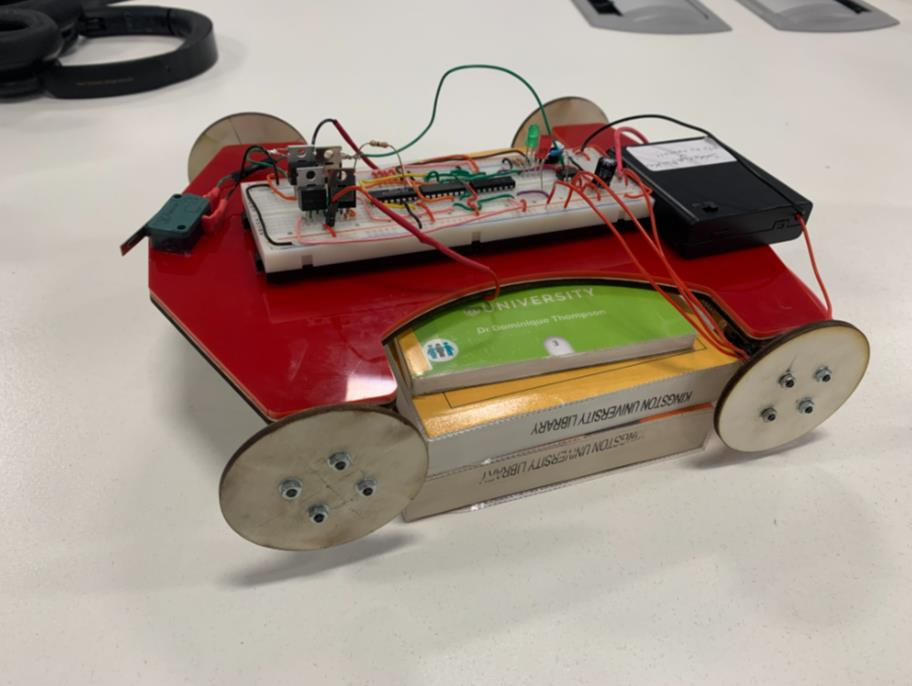
\includegraphics[width=0.7\textwidth]{extracted_images2/image_13_2.png}
\end{center}\vspace{0.6em}\noindent
The final design of the autonomous robotic charging device reflects a comprehensive integration of mechanical and electronic systems, ensuring optimal performance and reliability. The chassis, constructed from durable plywood and acrylic, provides a lightweight yet sturdy platform, while the use of plywood wheels and hubs minimizes friction and enhances mobility. Additionally, the strategic placement of the lead screw mechanism allows for precise positioning, ensuring the device can effectively navigate and connect to charging stations autonomously, thereby fulfilling the project's objectives


\newpage
\vspace*{-12pt}
\section{References}
\begin{enumerate}
	\item Imeche (2025). \textit{Design Challenge -Project Specification and Rules 2025 -V1.0 1 AUTOMATED EV CHARGING}. Available at: \url{https://www.imeche.org/docs/default-source/1-oscar/challenges/design-challenge/2025/imeche-design-challenge---project-specification-and-rules-2025---v1-0.pdf?sfvrsn=2}. 
\end{enumerate}

\end{document}
